\documentclass[11pt]{article}

\usepackage{ifpdf}
\usepackage{booktabs}
\usepackage{array}
\usepackage{paralist}
\usepackage{subfigure}
\usepackage[pdftex]{graphicx}
\usepackage{epstopdf}
\usepackage[cmex10]{amsmath}
\interdisplaylinepenalty=2500
\usepackage{geometry}
\geometry{letterpaper}
\usepackage{fancyhdr}
\pagestyle{fancy}
\renewcommand{\headrulewidth}{0pt}
\lhead{}\chead{}\rhead{}
\lfoot{}\cfoot{\thepage}\rfoot{}

\usepackage{amsfonts}
\usepackage{amstext}
\usepackage{booktabs}
\usepackage{threeparttable}
\usepackage{longtable}
\usepackage{listings}
\usepackage[font=normalsize]{caption}
\usepackage{textcomp}
\usepackage[usenames]{color}
\usepackage{soul}
\usepackage{fancyvrb}
\usepackage{relsize}
\usepackage[noadjust]{cite}
\usepackage{xr-hyper}
\usepackage[usenames,dvipsnames,svgnames,table]{xcolor}
\usepackage[colorlinks=true,urlcolor=blue,hyperfootnotes=false,backref=section,citecolor=LimeGreen]{hyperref}
\usepackage{upquote}
\usepackage[title,titletoc]{appendix}

\usepackage[nottoc,notlof,notlot]{tocbibind}
%\renewcommand{\FancyVerbFormatLine}[1]{\makebox[2mm][l]{}#1}
%\DefineVerbatimEnvironment%
%  {Code}{Verbatim}
%  {fontsize=\relsize{-1.5},
%  samepage=true,
%  frame=single}

\renewcommand{\FancyVerbFormatLine}[1]{\makebox[2mm][l]{}#1}
\DefineVerbatimEnvironment%
  {Notice}{Verbatim}
  {fontsize=\relsize{-1.5},
  samepage=true,
  xleftmargin=15mm,
  framesep=5mm,
  frame=single}

\newcommand{\covemda}{CoVEMDA}
\newcommand{\covemdagithuburl}{https://github.com/tamu-engineering-research/COVID-EMDA}
\newcommand{\matlab}{\textsc{MATLAB}}

\definecolor{BackgroundColor}{HTML}{e7f2fa}
\definecolor{SepColor}{HTML}{6ab0de}
\definecolor{DarkGreen}{rgb}{0.0,0.4,0.0}

\lstnewenvironment{Code}
    {\lstset{
        language=matlab,
        frame=shadowbox, 
        basicstyle=\ttfamily,
        commentstyle=\color{DarkGreen},
        stringstyle=\color{purple},
        keywordstyle=\bfseries\color{blue},
        backgroundcolor=\color{BackgroundColor}, 
        rulesepcolor=\color{SepColor}%
        }}
    {}

        
\def\sectionautorefname{Chapter}
\def\subsectionautorefname{Section}
\def\subsubsectionautorefname{Section}
\newcommand{\secref}[1]{\autoref{#1} \nameref{#1}}

\numberwithin{equation}{section}
\numberwithin{table}{section}
\renewcommand{\thetable}{\thesection\mbox{-}\arabic{table}}
\numberwithin{figure}{section}
\renewcommand{\thefigure}{\thesection\mbox{-}\arabic{figure}}



%%% title setting
\title{User's Manual for CoVEMDA Toolbox}
\author{}
\date{\today}
%\date{December 14, 2011\thanks{Second revision. First revision wyas December 13, 2011}} % comment this line to display the current date



%%% BEGIN DOCUMENT
\begin{document}
\maketitle
\thispagestyle{empty}
\newpage
\tableofcontents
\thispagestyle{empty}


%-------------------------------
\newpage
\setcounter{page}{1}
\section*{Website}
\addcontentsline{toc}{section}{Website}

\url{https://github.com/tamu-engineering-research/COVID-EMDA}

\begin{center}
	\noindent
\includegraphics[width=0.5\textwidth]{figures/covid_emda_logo.JPG}
\end{center}



%-------------------------------
\newpage
\section{Introduction} \label{sec:intro}

\subsection{Background}

\subsection{Features}

\subsection{Support Team}

\subsection{Suggested Citation}

\subsection{License}
The code of \covemda~is licensed under the \textbf{MIT License}, the full text of which can be found at the top level of distribution or \url{https://github.com/tamu-engineering-research/COVID-EMDA/blob/master/LICENSE} and reads as follows.
\begin{Notice}
Copyright (c) 2020 Guangchun Ruan

Permission is hereby granted, free of charge, to any person obtaining a copy
of this software and associated documentation files (the "Software"), to deal
in the Software without restriction, including without limitation the rights
to use, copy, modify, merge, publish, distribute, sublicense, and/or sell
copies of the Software, and to permit persons to whom the Software is
furnished to do so, subject to the following conditions:

The above copyright notice and this permission notice shall be included in all
copies or substantial portions of the Software.

THE SOFTWARE IS PROVIDED "AS IS", WITHOUT WARRANTY OF ANY KIND, EXPRESS OR
IMPLIED, INCLUDING BUT NOT LIMITED TO THE WARRANTIES OF MERCHANTABILITY,
FITNESS FOR A PARTICULAR PURPOSE AND NONINFRINGEMENT. IN NO EVENT SHALL THE
AUTHORS OR COPYRIGHT HOLDERS BE LIABLE FOR ANY CLAIM, DAMAGES OR OTHER
LIABILITY, WHETHER IN AN ACTION OF CONTRACT, TORT OR OTHERWISE, ARISING FROM,
OUT OF OR IN CONNECTION WITH THE SOFTWARE OR THE USE OR OTHER DEALINGS IN THE
SOFTWARE.
\end{Notice}






%-------------------------------
\newpage
\section{Getting Started} \label{sec:start}

\subsection{System Requirements}
To use \covemda~Toolbox you will need: MATLAB\textsuperscript{\tiny \textregistered} version 9.8 (R2020a). 

\small\emph{
\begin{enumerate}[NOTE.1]
    \item Despite the fact that \textnormal{GNU Octave} can also tackle \textsf{.m} files, several functions like \textsf{isdatetime}  have not been implemented in \textnormal{GNU Octave} (even the latest 6.1.0).
    \item For those who want long-term data support, \textnormal{Git}\footnote{``Git is a free and open-source distributed version control system.'' It can guarantee you the easy access to the latest released data in multiple platforms. Git is available on its \href{https://git-scm.com/}{official website}, where both command-line version and gui version are provided.}/\textnormal{GitHub Desktop}\footnote{``GitHub Desktop extends and simplifies your Git and GitHub workflow using a visual interface.'' Only systems of macOS and Windows are supported. The software is accessible at \url{https://desktop.github.com/}, while docs are available at \url{https://docs.github.com/en/desktop}} are needed for your latter convenience.
\end{enumerate}    
}

As for the hardware requirements, please refer to the System Requirements of MATLAB according to the specific version\footnote{\url{https://www.mathworks.com/support/requirements/previous-releases.html}}.

\subsection{Getting Data and Toolbox}
Both data hub and toolbox are provided in the distribution. 
You can get our data hub and toolbox for a specific version, by either cloning the repository to your local disk or downloading the whole repository zip-file at a time. However, the latter is not recommended to users that want to keep data updated daily.
\subsubsection{Clone the repository to your local disk.}
    \begin{itemize}
        \item \textbf{Git} required. Open the \textbf{Git Bash} at certain file folder (the one you want the software to be placed in) and type the following command:

\verb!git clone https://github.com/tamu-engineering-research/COVID-EMDA.git!

        \item Or if you are unfamiliar with \textbf{Git Bash}, open \textbf{Git GUI} and 
        \begin{enumerate}
            \item Click the \textbf{Clone Existing Repository} button.
            
            \begin{figure}[htbp]
                \centering
                \caption{Step.1}
                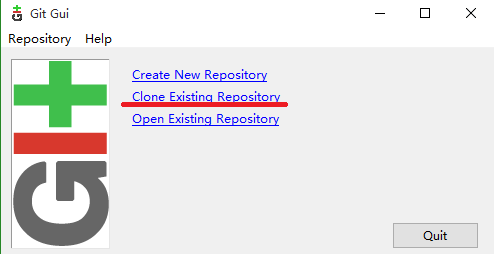
\includegraphics[width=.7\textwidth]{figures/git_gui_step_1.png}
            \end{figure}

            \item Type in ``https://github.com/tamu-engineering-research/COVID-EMDA.git'' in Source Location.
            \item Choose the local folder of your project, e.g. \verb!My Project! under disk G.
            
            \begin{figure}[htbp]
                \centering
                \caption{Step.2}
                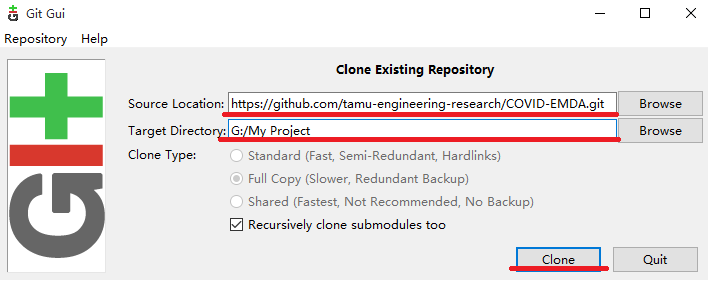
\includegraphics[width=.7\textwidth]{figures/git_gui_step_2.png}
            \end{figure}

            \item Click the \textbf{Clone} button.
    
            \begin{figure}[htbp]
                \centering
                \caption{Step.3}
                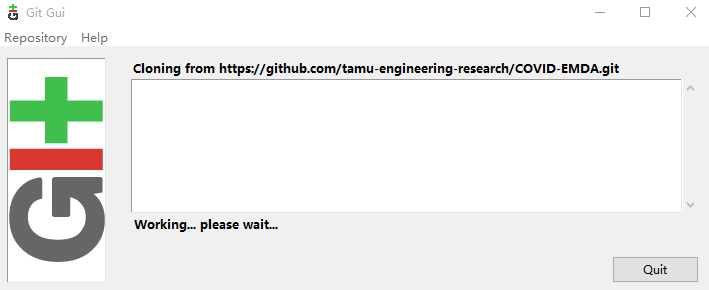
\includegraphics[width=.7\textwidth]{figures/git_gui_step_3.png}
            \end{figure}

        \end{enumerate}

        \item \textbf{Github Desktop} required. 
        \begin{enumerate}
            \item Click \textbf{Clone repository...} under the \textbf{File} menu bar. 
            \begin{figure}[htbp]
                \centering
                \caption{Clone}
                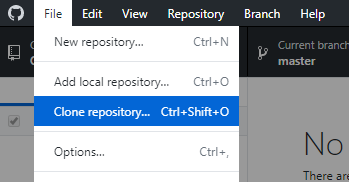
\includegraphics[width=.7\textwidth]{figures/github_desktop_step_1.png}
            \end{figure}
            \item Choose \textbf{URL} and input \verb!username/repository! as follows: 
            
            \verb!tamu-engineering-research/COVID-EMDA!

            \begin{figure}[htbp]
                \centering
                \caption{Path}
                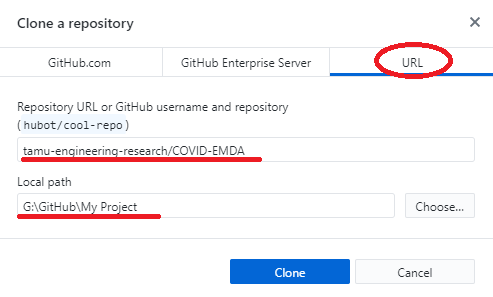
\includegraphics[width=.7\textwidth]{figures/github_desktop_step_2.png}
            \end{figure}

            \item Choose your local repository path and click \textbf{Clone}.
            \begin{figure}[htbp]
                \centering
                \caption{Cloning}
                
\includegraphics[width=.7\textwidth]{figures/github_desktop_step_3.png}
            \end{figure}
        \end{enumerate}
        
    \end{itemize} 
\subsubsection{Download the zip-file.}
    \begin{itemize}
        \item Go to \href{\covemdagithuburl}{\covemda~GitHub Repository}.
        \item Click the green \textbf{Code} button.
        \item Click the \textbf{Download ZIP} button.
        \item Uncompress the zip file to certain directory.
        \begin{figure}[htbp]
            \centering
            \caption{Download from GitHub Website}
            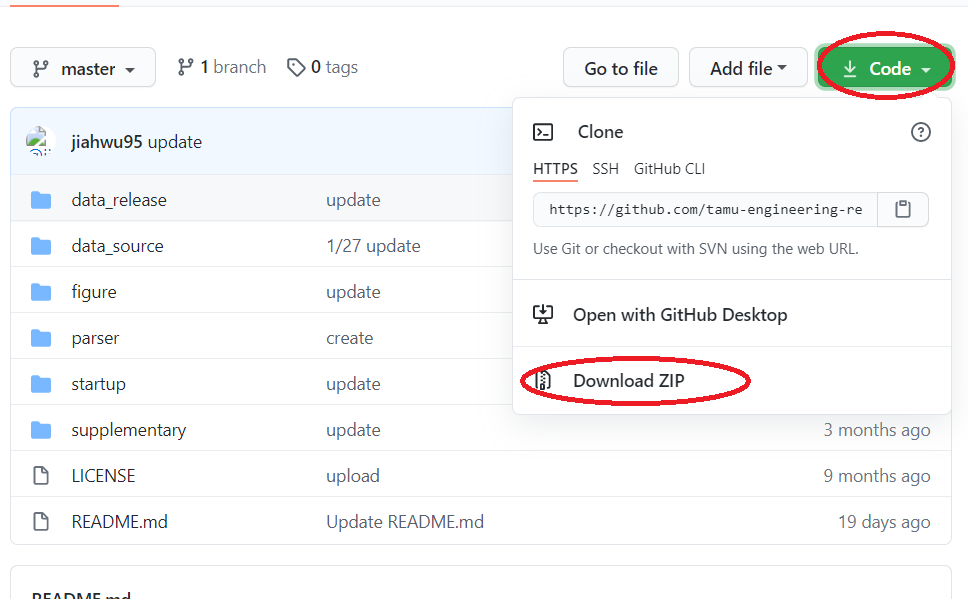
\includegraphics{figures/github_website_step_1.png}
        \end{figure}
    \end{itemize}

\subsection{Running an Example}





%----------------------------------------
\newpage
\section{Data Hub} \label{sec:datahub}

\subsection{Data Category}

\subsection{Data Structure}

\subsection{Field Description}

\subsection{Quality Control}








%--------------------------------------------
\newpage
\section{Visualization} \label{sec:visual}

\subsection{Generation Mix}
\subsubsection{plot generation mix}
\begin{Code}
  ar = plot_generation_mix(market,Name,Value)
\end{Code}

Plot the generation mix of a market.

Return the area objects of the plot, which represents the proportion of all fuel types over time.

This function is based on \matlab{} function \verb!area!.


\paragraph{Input Arguments}
\subparagraph{market:} \textit{character vectors}

Name of the market, specified as one of the seven market names:

\verb!'caiso' | 'ercot' | 'isone' | 'miso' | 'nyiso' | 'pjm' | 'spp'!

\paragraph{Name-Value Pair Arguments}
\subparagraph{DateRange:} \textit{datetime array $|$ string array $|$ cell array of character vectors}

Range of time, specified as a datetime array, a string array or a cell array of character vectors. Default \verb!{'2017-01-01','2020-07-15'}!.

Example: \verb!{'2017-01-01','2020-07-15'}!

Example: \verb!["2020-02-01","2020-04-30"]!

\subparagraph{ResampleBin:} \textit{string $|$ character vector}

Binning scheme for resampling. See also \verb!groupsummary!. Default \verb!'month'!.

\subparagraph{ColorMap:} \textit{table $|$ structure array $|$ string array $|$ cell array of character vectors}

Colors of all the areas in the plot. See also \verb!Area Properties!. Default:

\verb!["coal","gas","oil","nuclear","hydro","wind","solar","other","import";!

\verb!"#a67a6d","#f69850","#b35711","#3f9b98","#a0d8f1","#73c698","#ffbd4a",!

\verb!"#b4b4b4","white"]!

\subparagraph{Others:}

Modifications of the area objects. See \verb!Area Properties!.



\paragraph{Output Arguments}
\subparagraph{ar:} \textit{area objects}

Area objects of the plot. The number of objects is equal to the number of fuel types. Use \verb!ar! to modify properties of the areas after creating them. See also \verb!Area Properties!.



\paragraph{Examples}
\subparagraph{Plot generation mix of a market}

Calculate the generation mix of SPP. Display it in an area plot.

\begin{Code}
  plot_generation_mix('spp');
\end{Code}

\begin{center}
  \noindent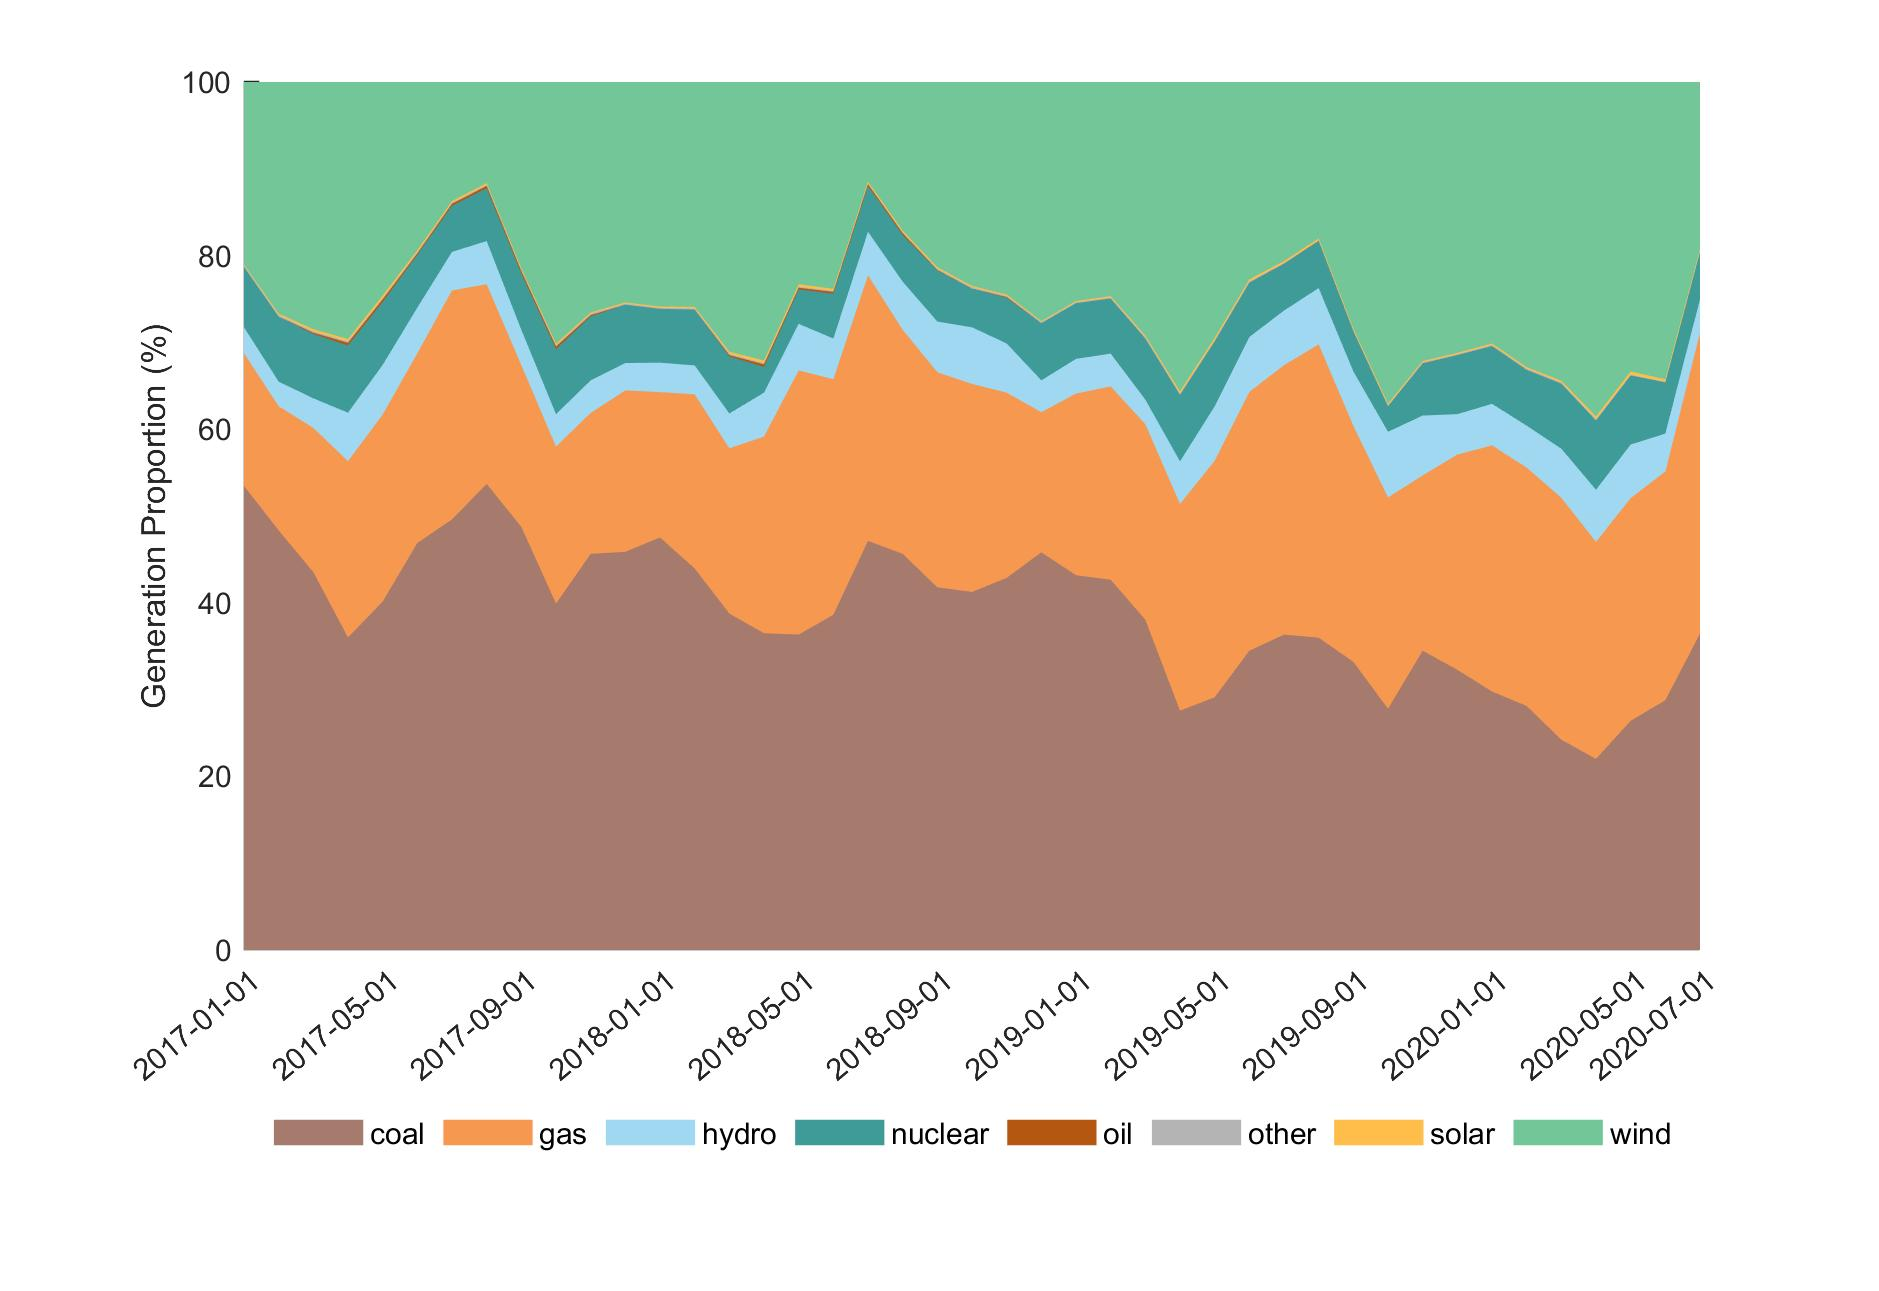
\includegraphics[width=\textwidth]{figures/plot_generation_mix_example1.jpg}
\end{center}

\subparagraph{Customize binning scheme}

Calculate the everyday generation mix of SPP in Jan-2020. Display it in an area plot.

\begin{Code}
  plot_generation_mix('spp', 'DateRange',...
  {'2020-01-01','2020-01-31'}, 'ResampleBin', 'day');
\end{Code}

\begin{center}
  \noindent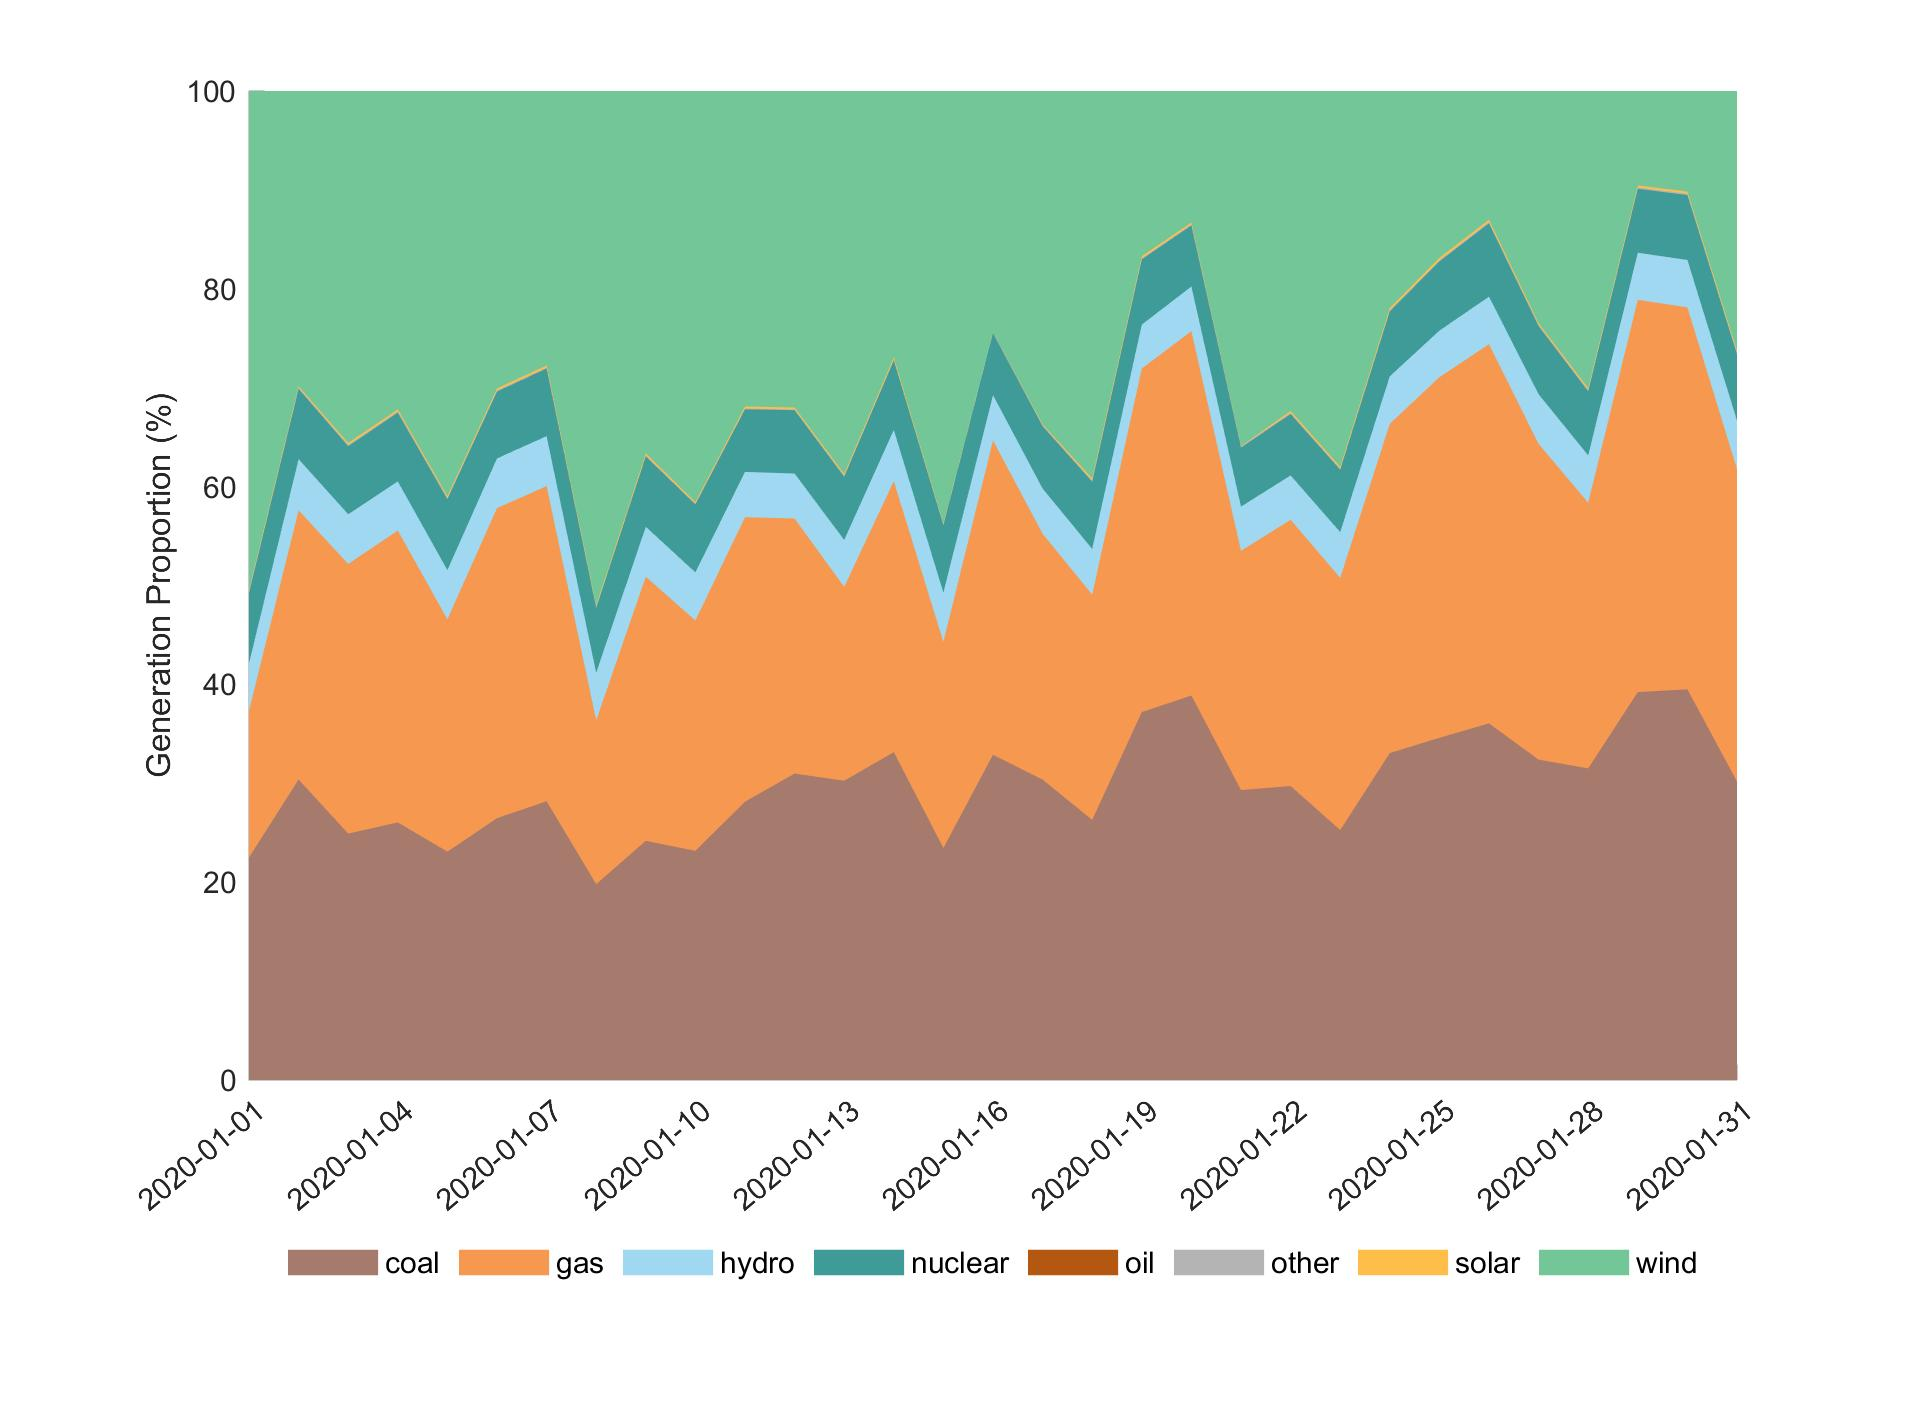
\includegraphics[width=\textwidth]{figures/plot_generation_mix_example2.jpg}
\end{center}

\subparagraph{Customize color map}
Calculate the generation mix of SPP. Display it in an area plot with specified color map.

\begin{Code}
  ColorMap = ["coal",    "#0072BD";
  "gas",     "#D95319";
  "oil",     "#EDB120";
  "nuclear", "#7E2F8E";
  "hydro",   "#77AC30";
  "wind",    "#4DBEEE";
  "solar",   "#A2142F";
  "other",   "green";
  "import",  "white"]';
  plot_generation_mix('spp', 'ColorMap', ColorMap);
\end{Code}

\begin{center}
  \noindent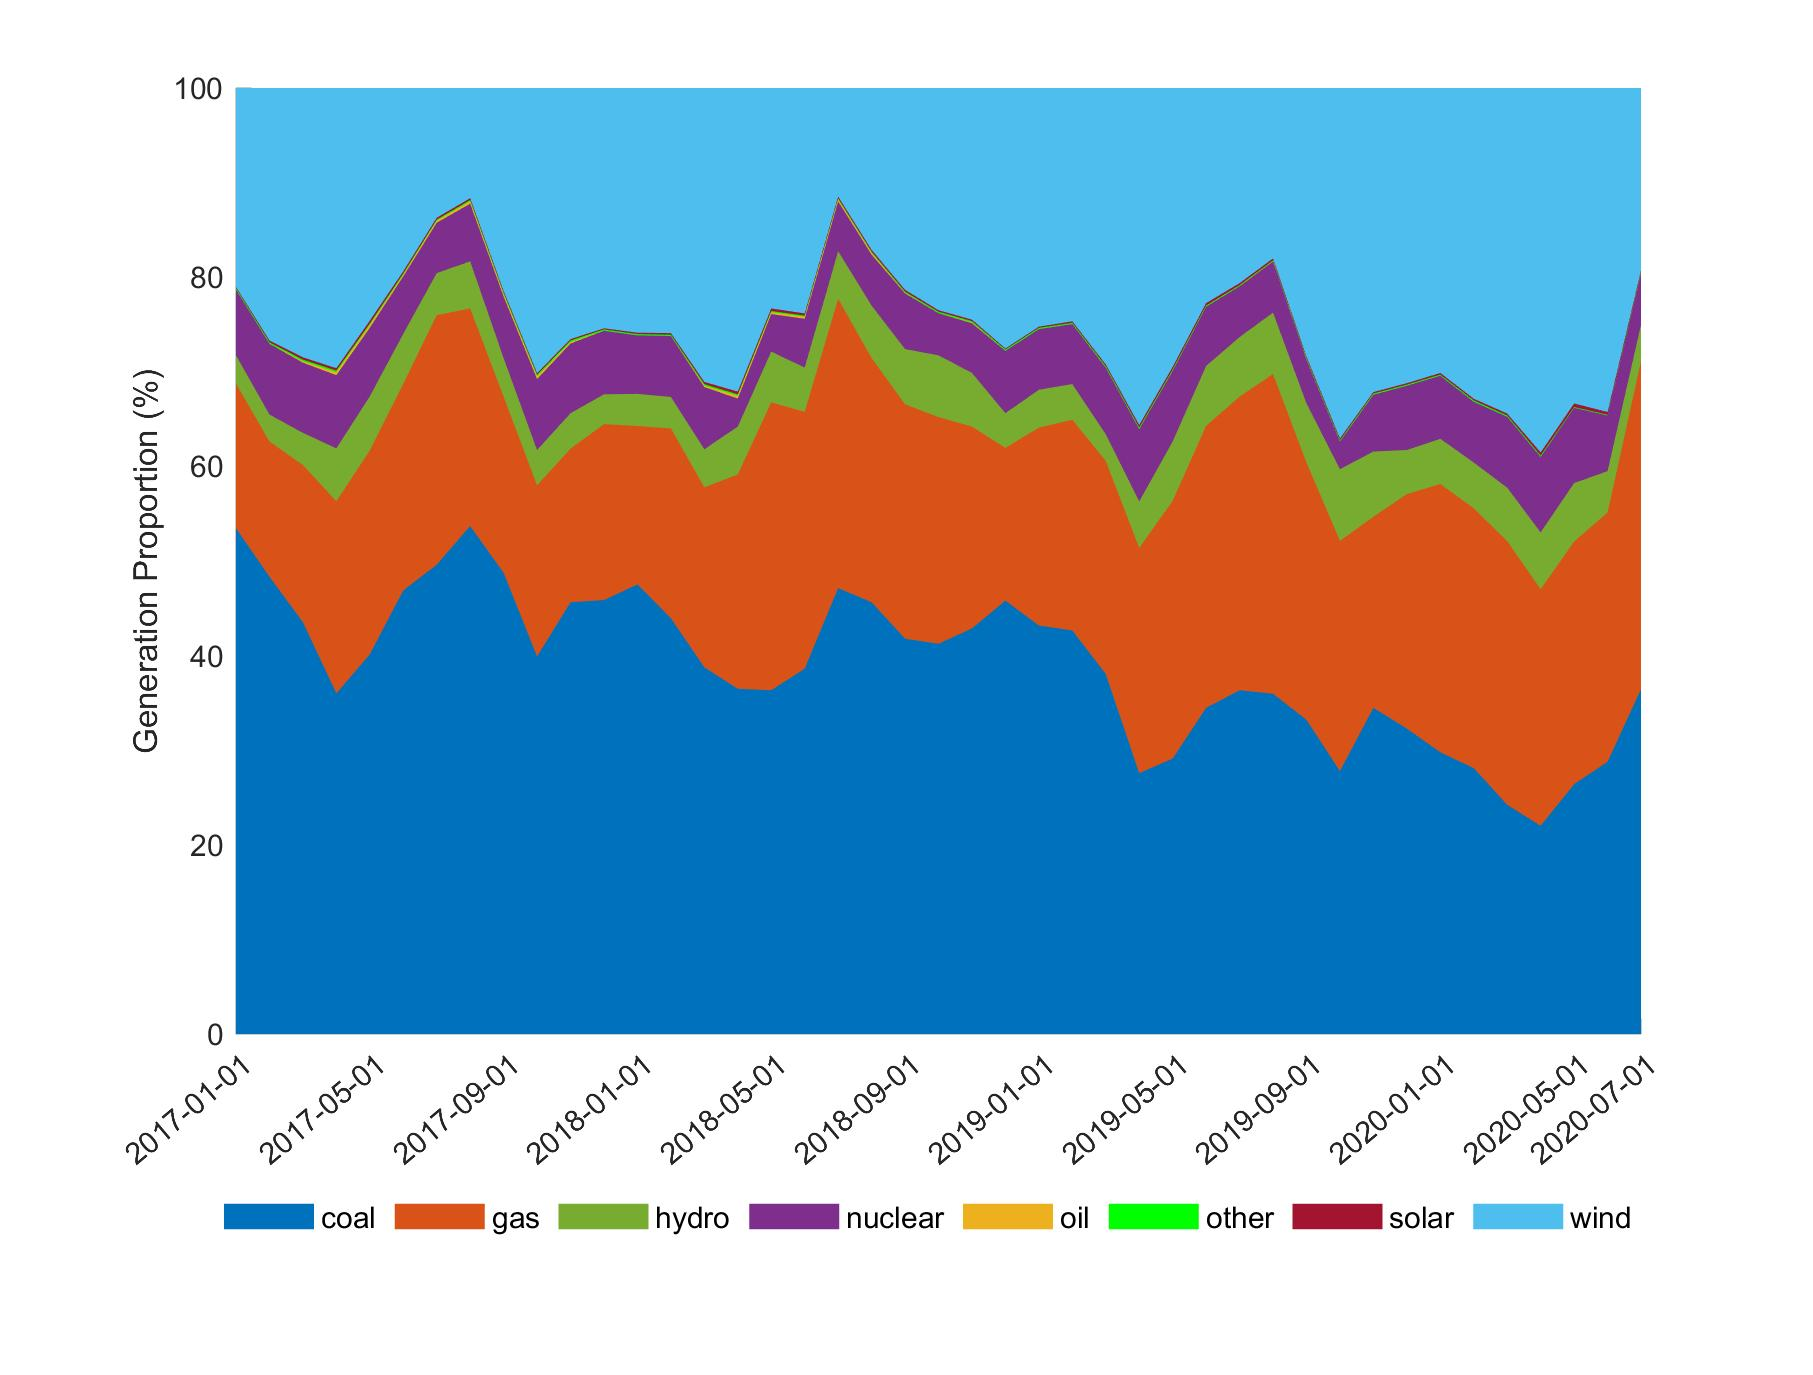
\includegraphics[width=\textwidth]{figures/plot_generation_mix_example3.jpg}
\end{center}

\subparagraph{Specify area properties}
Calculate the generation mix of SPP. Display it in an area plot and visualize the edges.

\begin{Code}
  plot_generation_mix('spp',...
  'ResampleBin', 'month', 'EdgeColor',...
  'black', 'LineStyle', '--');
\end{Code}

\begin{center}
  \noindent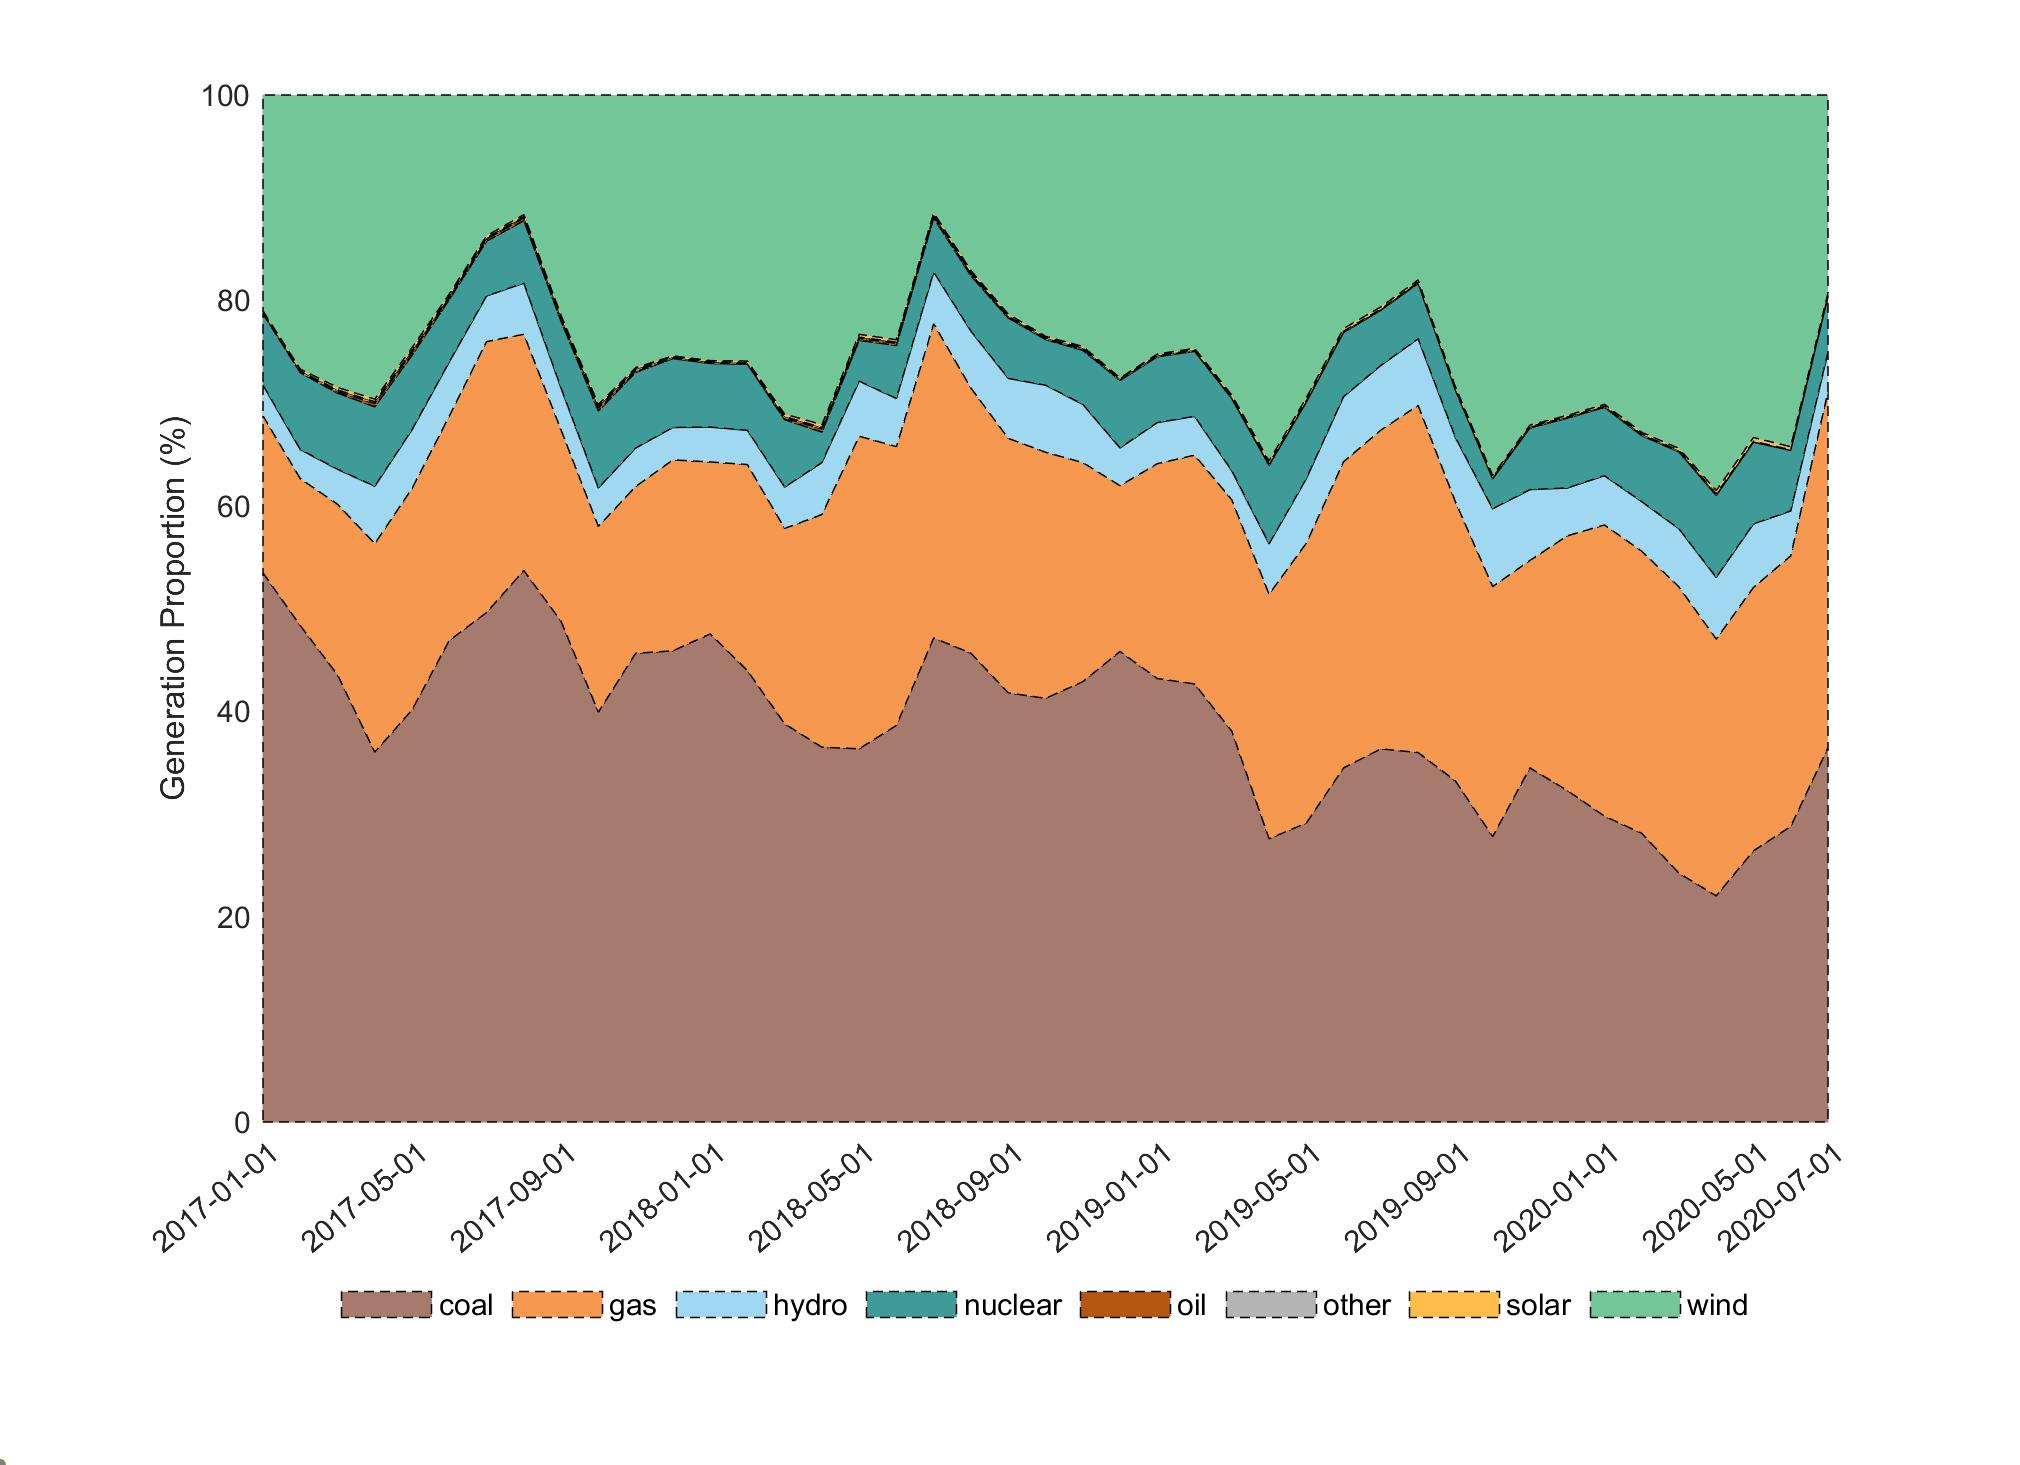
\includegraphics[width=\textwidth]{figures/plot_generation_mix_example4.jpg}
\end{center}

\subparagraph{Modify properties after plotting}
Calculate the generation mix of SPP. Modify the properties of area objects and axes after displaying the plot.

\begin{Code}
  ar = plot_generation_mix('spp');
  ar(1).EdgeColor = 'black';
  ar(1).LineWidth = 2;
  ar(end).FaceAlpha = 0.5;
  ax = gca;
  ax.FontSize = 15;
\end{Code}

Note that \verb!ar! usually contains more than one area objects (one for each fuel type), and they can be modified individually. Also, customize the axes by using \verb!ax = gca!.

For a list of properties, see \verb!Area Properties! and \verb!Axes Properties!.

\begin{center}
  \noindent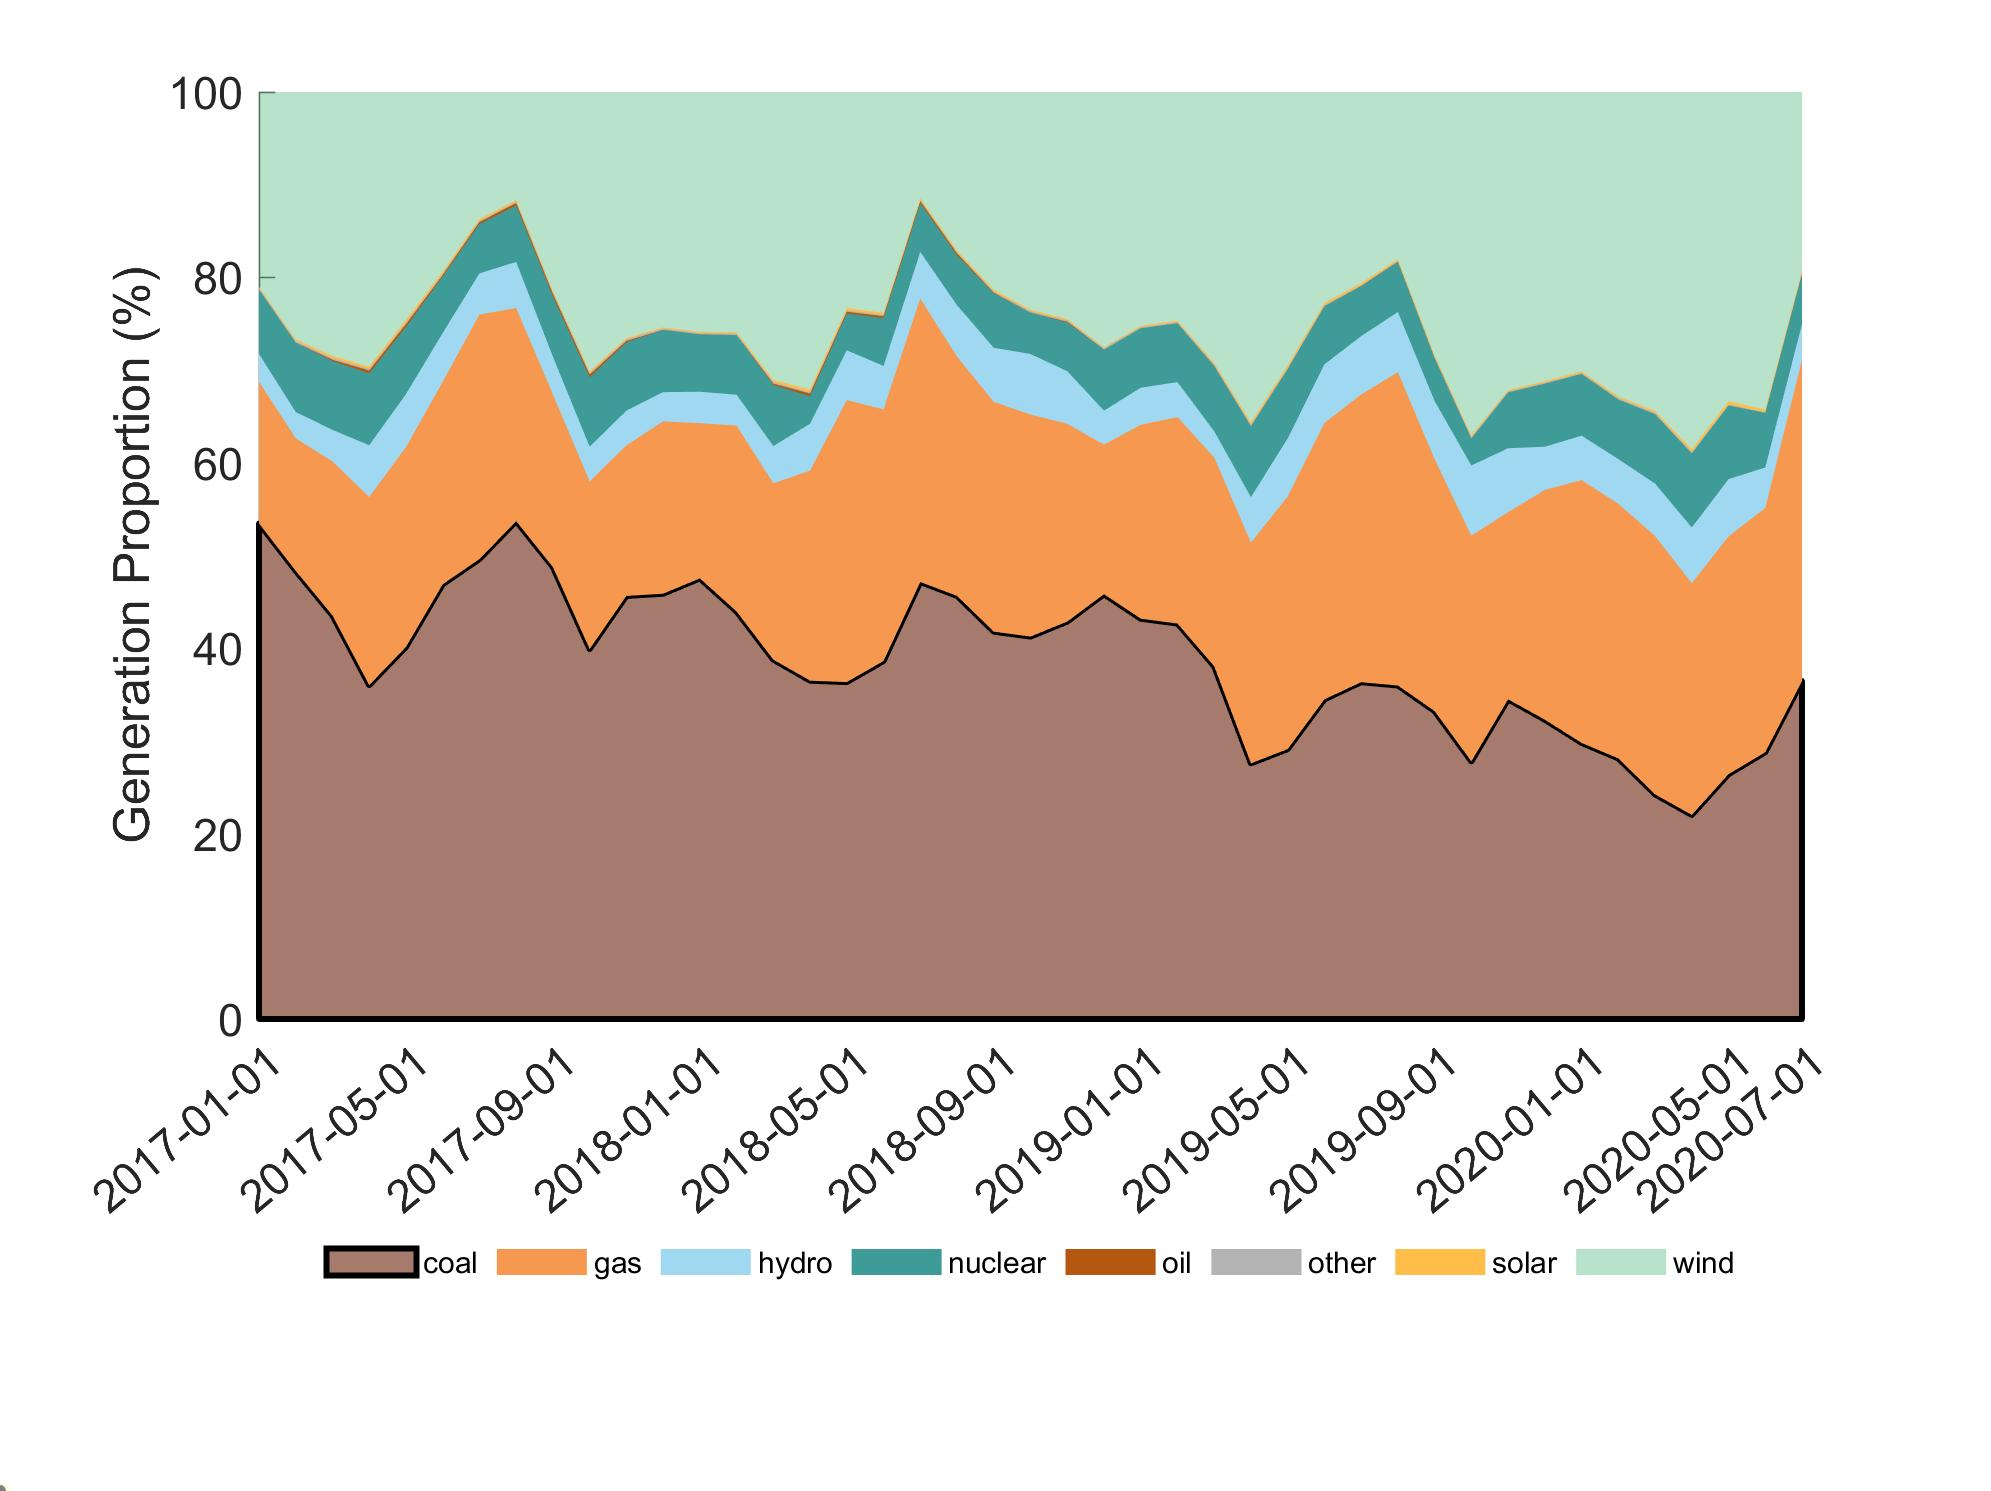
\includegraphics[width=\textwidth]{figures/plot_generation_mix_example5.jpg}
\end{center}





\subsection{Renewable Energy}
\subsubsection{plot renewable share}
\begin{Code}
  p = plot_renewable_share(market,Name,Value)
\end{Code}

Plot the renewable share curve of a market for a specified date range.

Return the line objects of the plot, which represents the renewable proportion over time.



\paragraph{Input Arguments}
\subparagraph{market:} \textit{character vectors}

Name of the market, specified as one of the seven market names:

\verb!'caiso' | 'ercot' | 'isone' | 'miso' | 'nyiso' | 'pjm' | 'spp'!

\paragraph{Name-Value Pair Arguments}
\subparagraph{DateRange:} \textit{datetime array $|$ string array $|$ cell array of character vectors}

Range of time, specified as a datetime array, a string array or a cell array of character vectors. Default \verb!{'2017-01-01','2020-07-15'}!.

Example: \verb!{'2017-01-01','2020-07-15'},["2018-02-01","2018-02-28"]!

\subparagraph{ResampleBin:} \textit{string $|$ character vector}

Binning scheme. See also \verb!groupsummary!. Default \verb!'none'!.
\subparagraph{ResampleMethod:} \textit{string $|$ character vector}

Method scheme. See also \verb!groupsummary!. Default \verb!'mean'!.

\subparagraph{Color:} \textit{string $|$ character vector}

Color scheme. See also \verb!groupsummary!. Default \verb!'#0072BD'!.

\subparagraph{Others:}

Modifications of the line objects. See \verb!Line Properties!.



\paragraph{Output Arguments}
\subparagraph{p:} \textit{line objects}

Line objects of the graph. Use \verb!line! to modify properties of the line after creating them. See also \verb!Line Properties!.



\paragraph{Examples}
\subparagraph{Plot renewable share of a market}

Calculate the generation mix of NYISO. Display it in an area plot.

\begin{Code}
  plot_renewable_share('nyiso');
\end{Code}

\begin{center}
  \noindent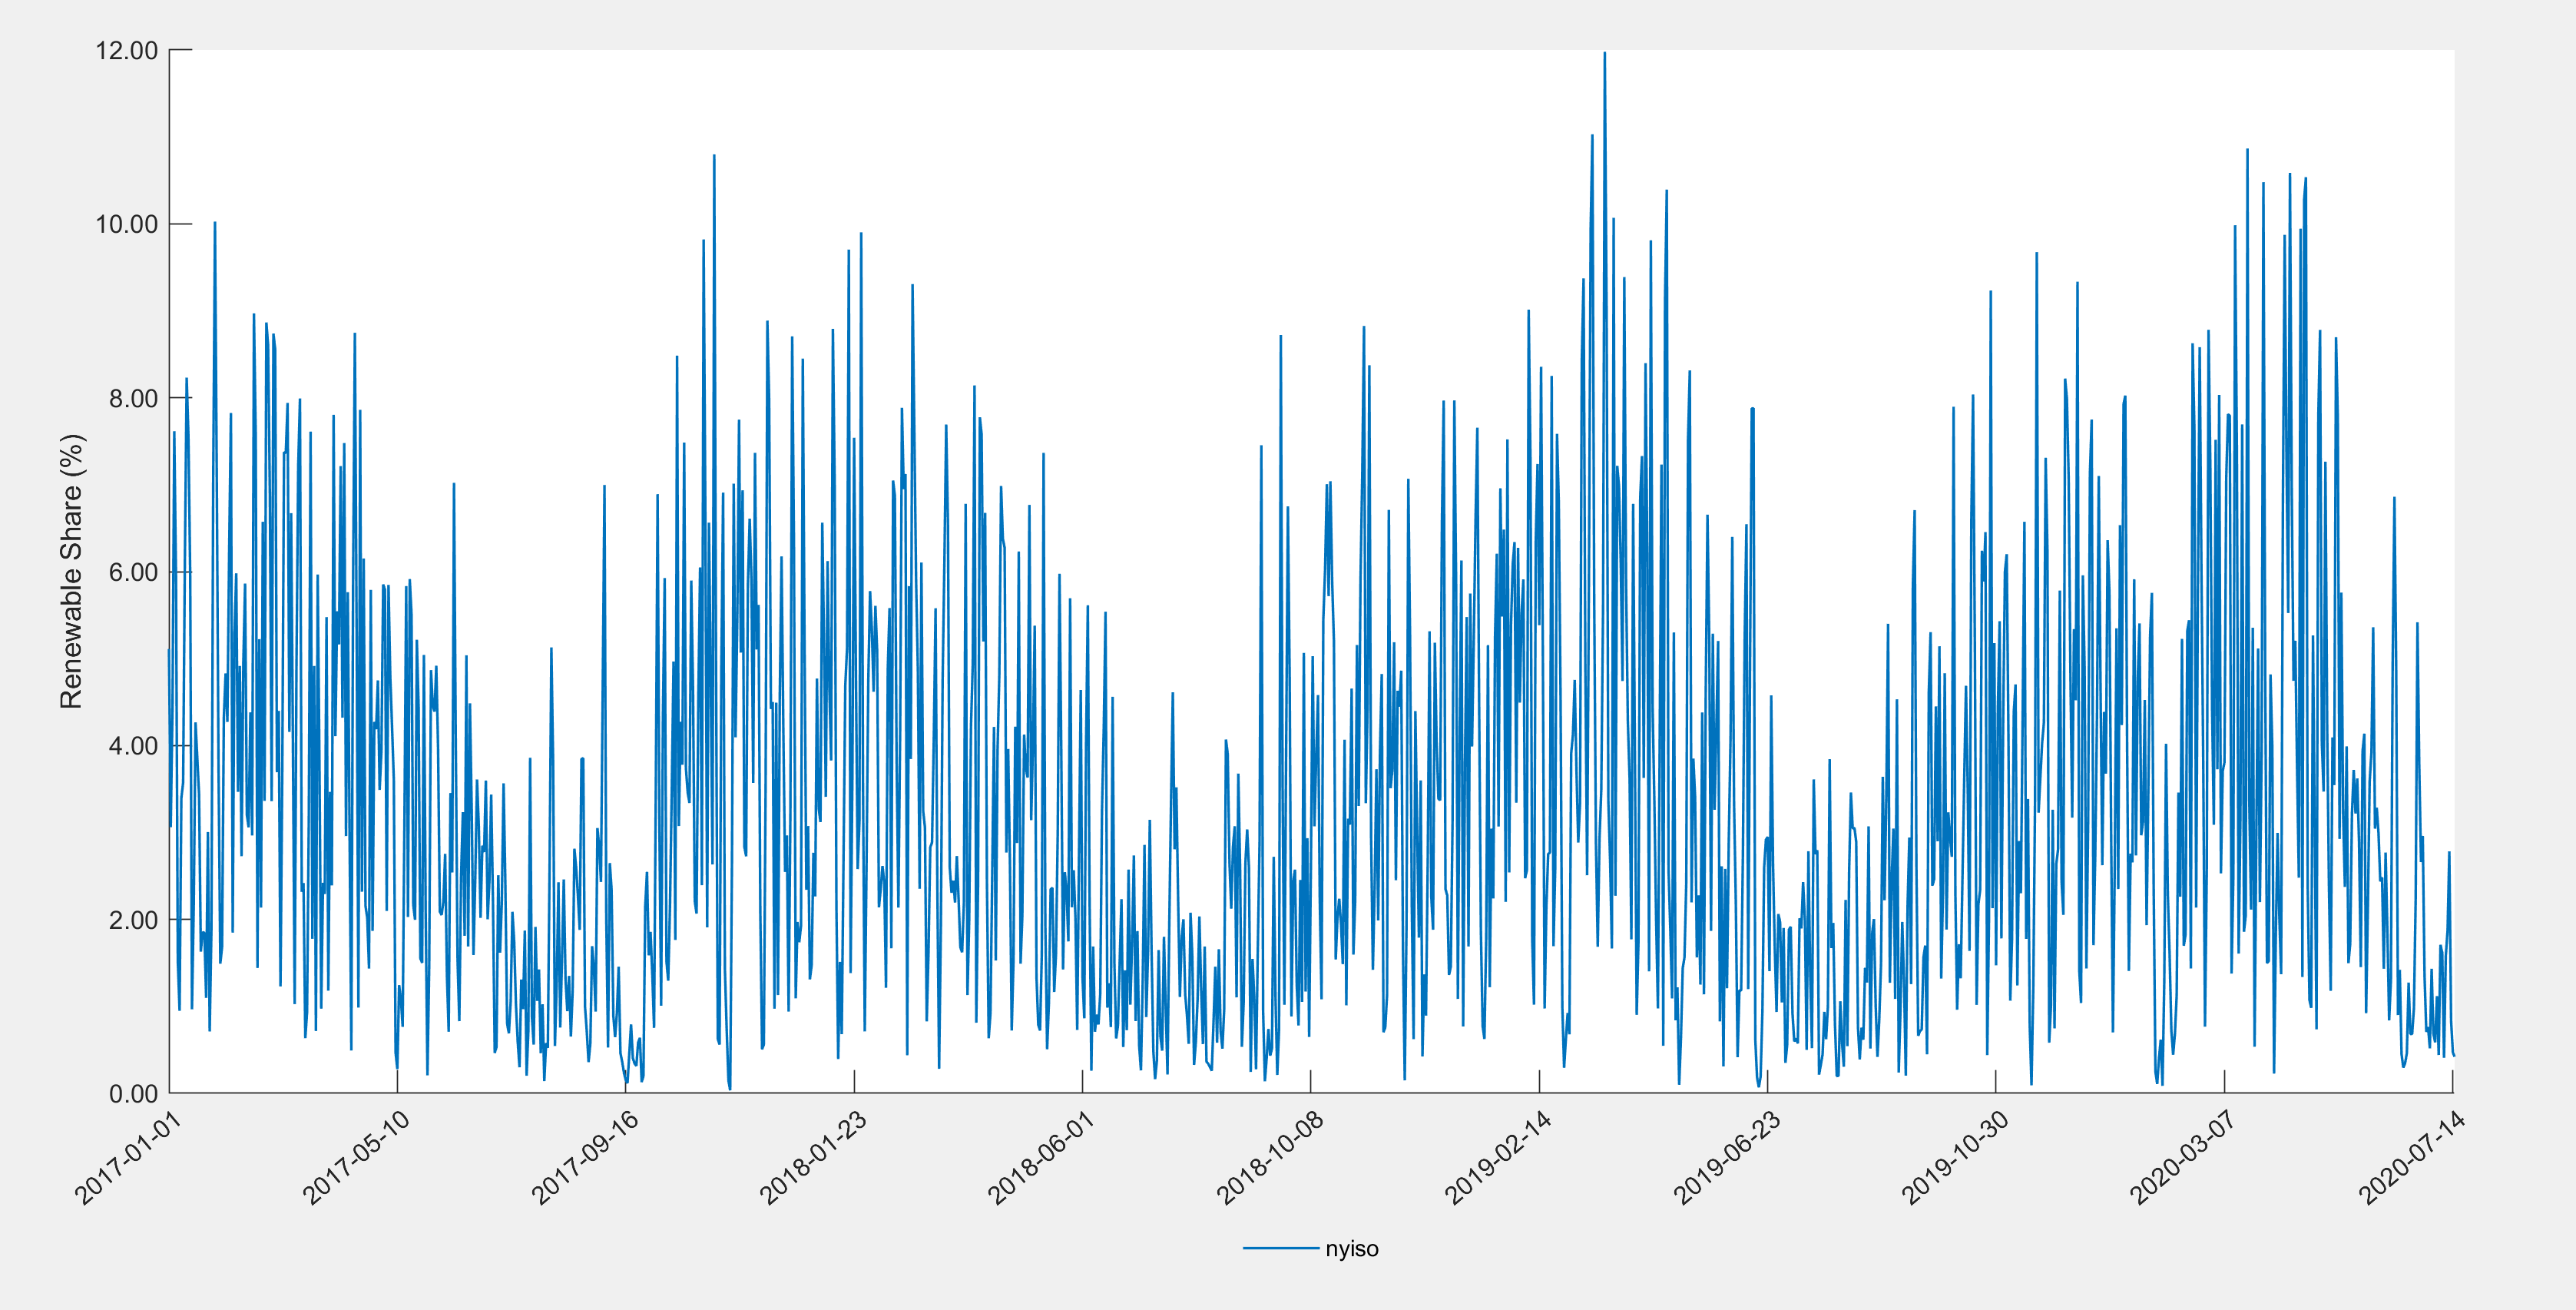
\includegraphics[width=\textwidth]{figures/plot_renewable_share_example1.jpg}
\end{center}

\subparagraph{Customize binning scheme}

Calculate the every month renewable share of NYISO from Jan 1$^{st}$-2017 to July 15$^{th}$-2020. Display it in an area plot.

\begin{Code}
  plot_renewable_share('nyiso', 'DateRange', ...
  {'2017-01-01', '2020-07-15'},'ResampleBin', 'month');
\end{Code}

\begin{center}
  \noindent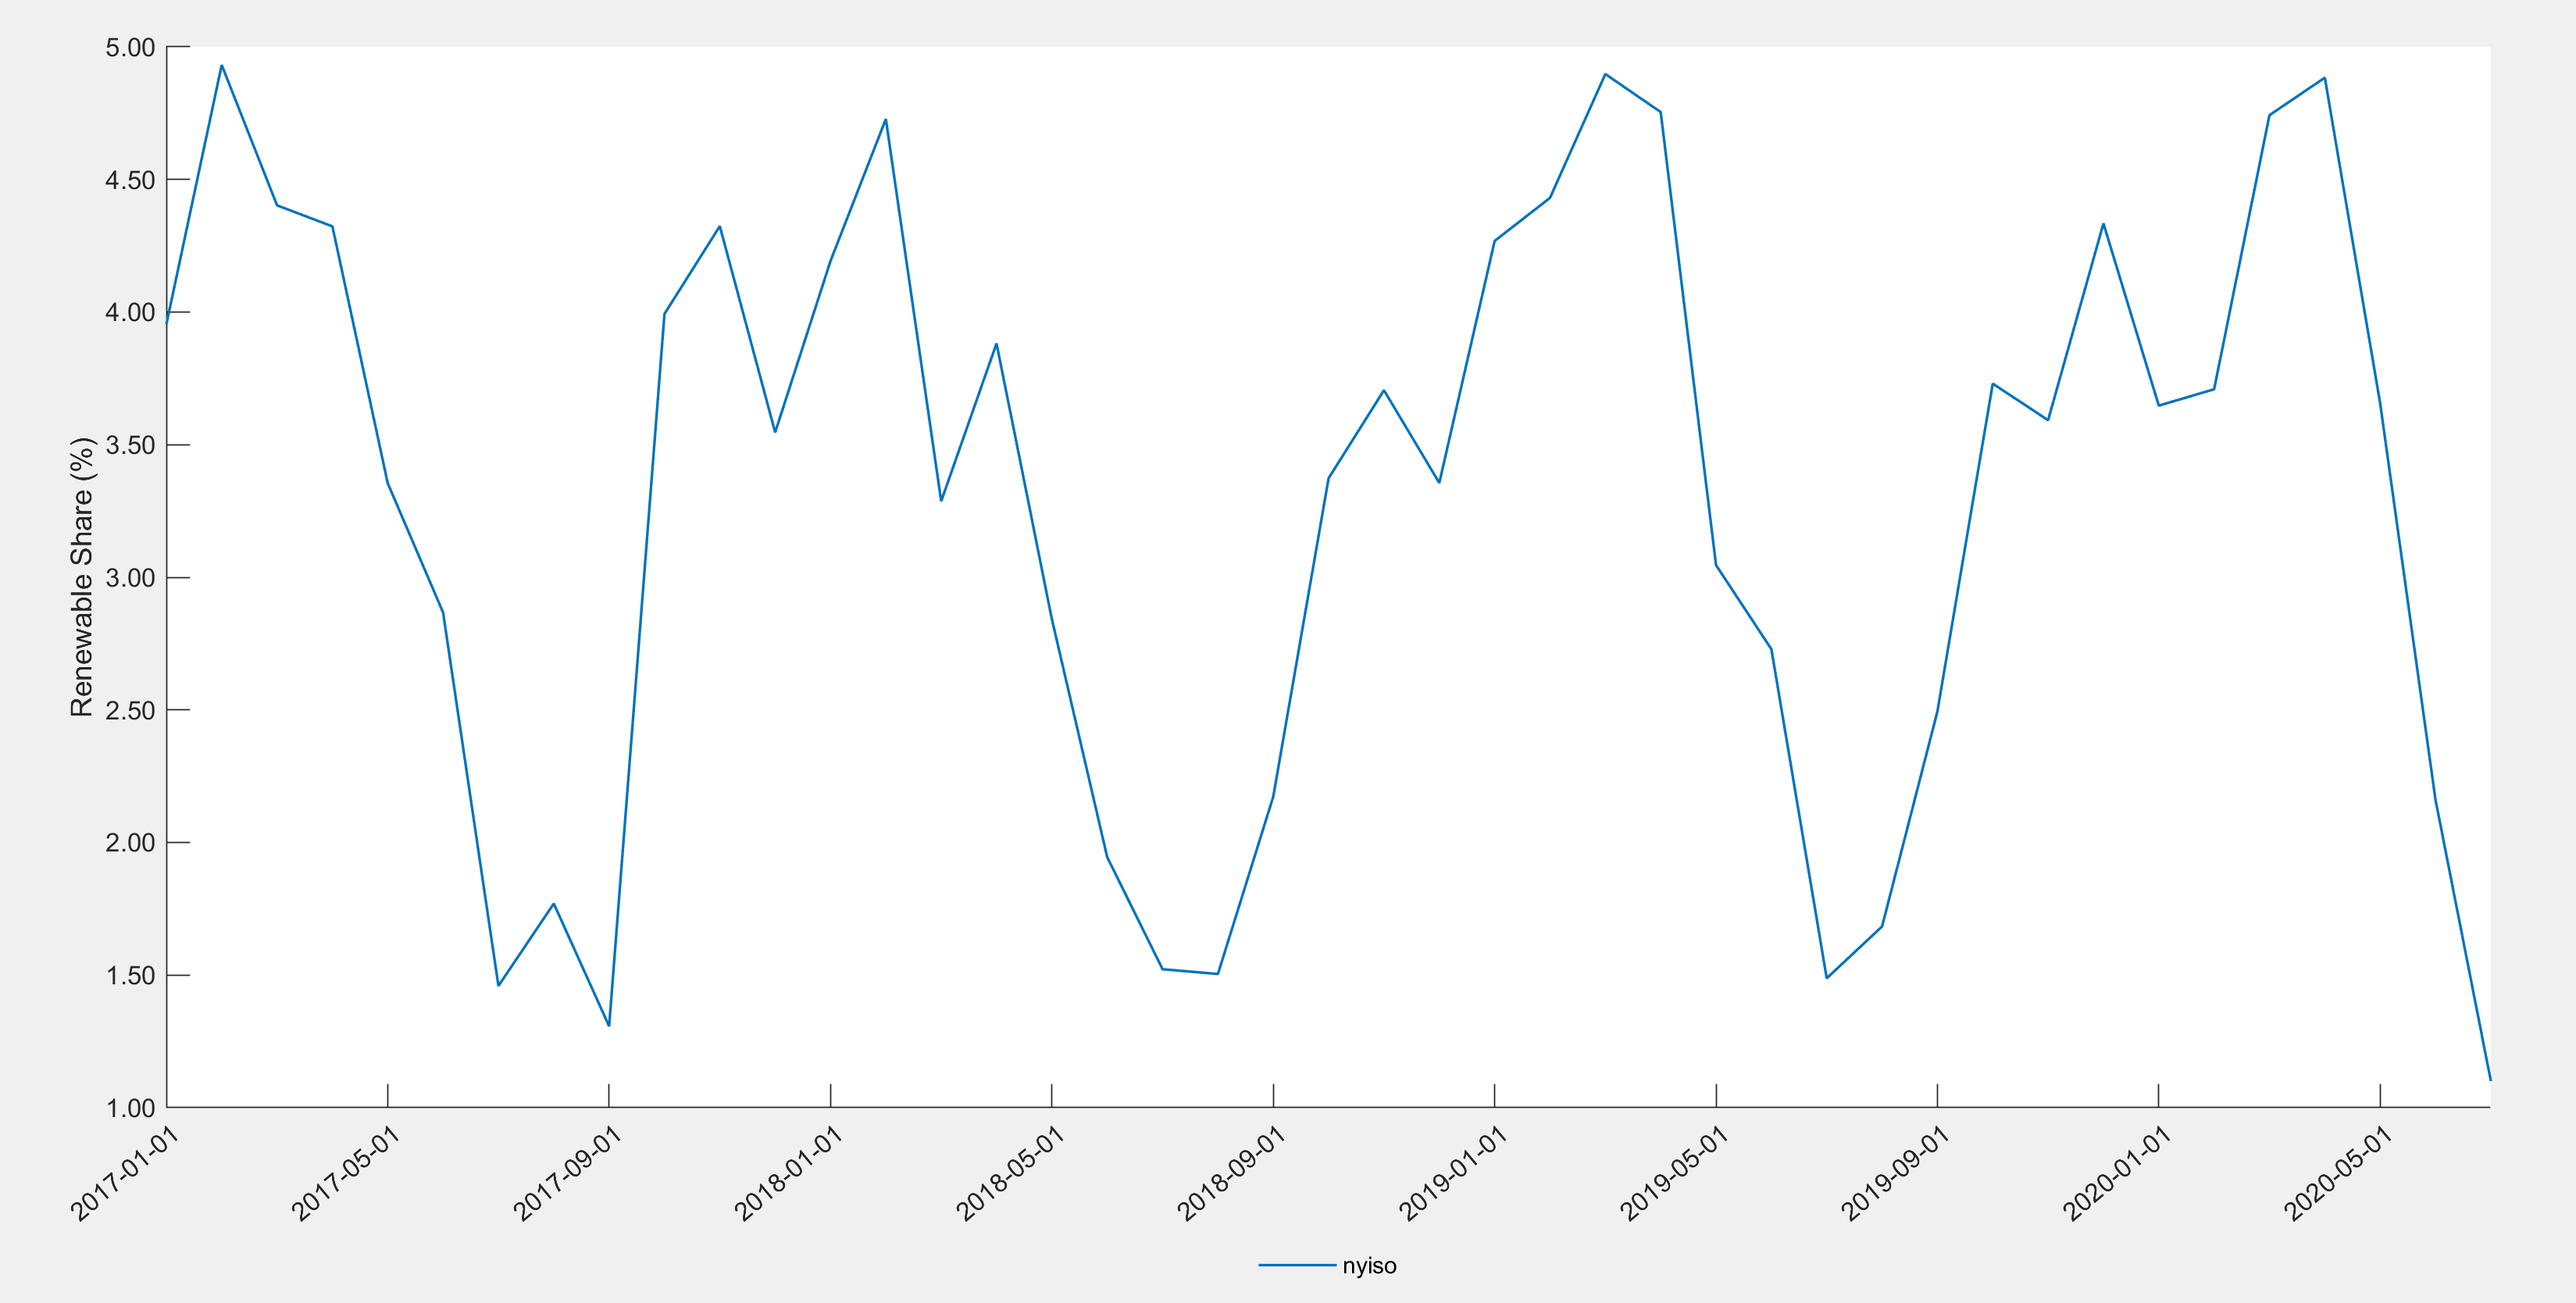
\includegraphics[width=\textwidth]{figures/plot_renewable_share_example2.jpg}
\end{center}

\subparagraph{Customize color}
Calculate the renewable share of NYISO. Display it in an line plot with specified color.

\begin{Code}
  plot_renewable_share('nyiso', 'DateRange', ...
  {'2020-02-01', '2020-04-30'},'Color', '#A2142F');
\end{Code}

\begin{center}
  \noindent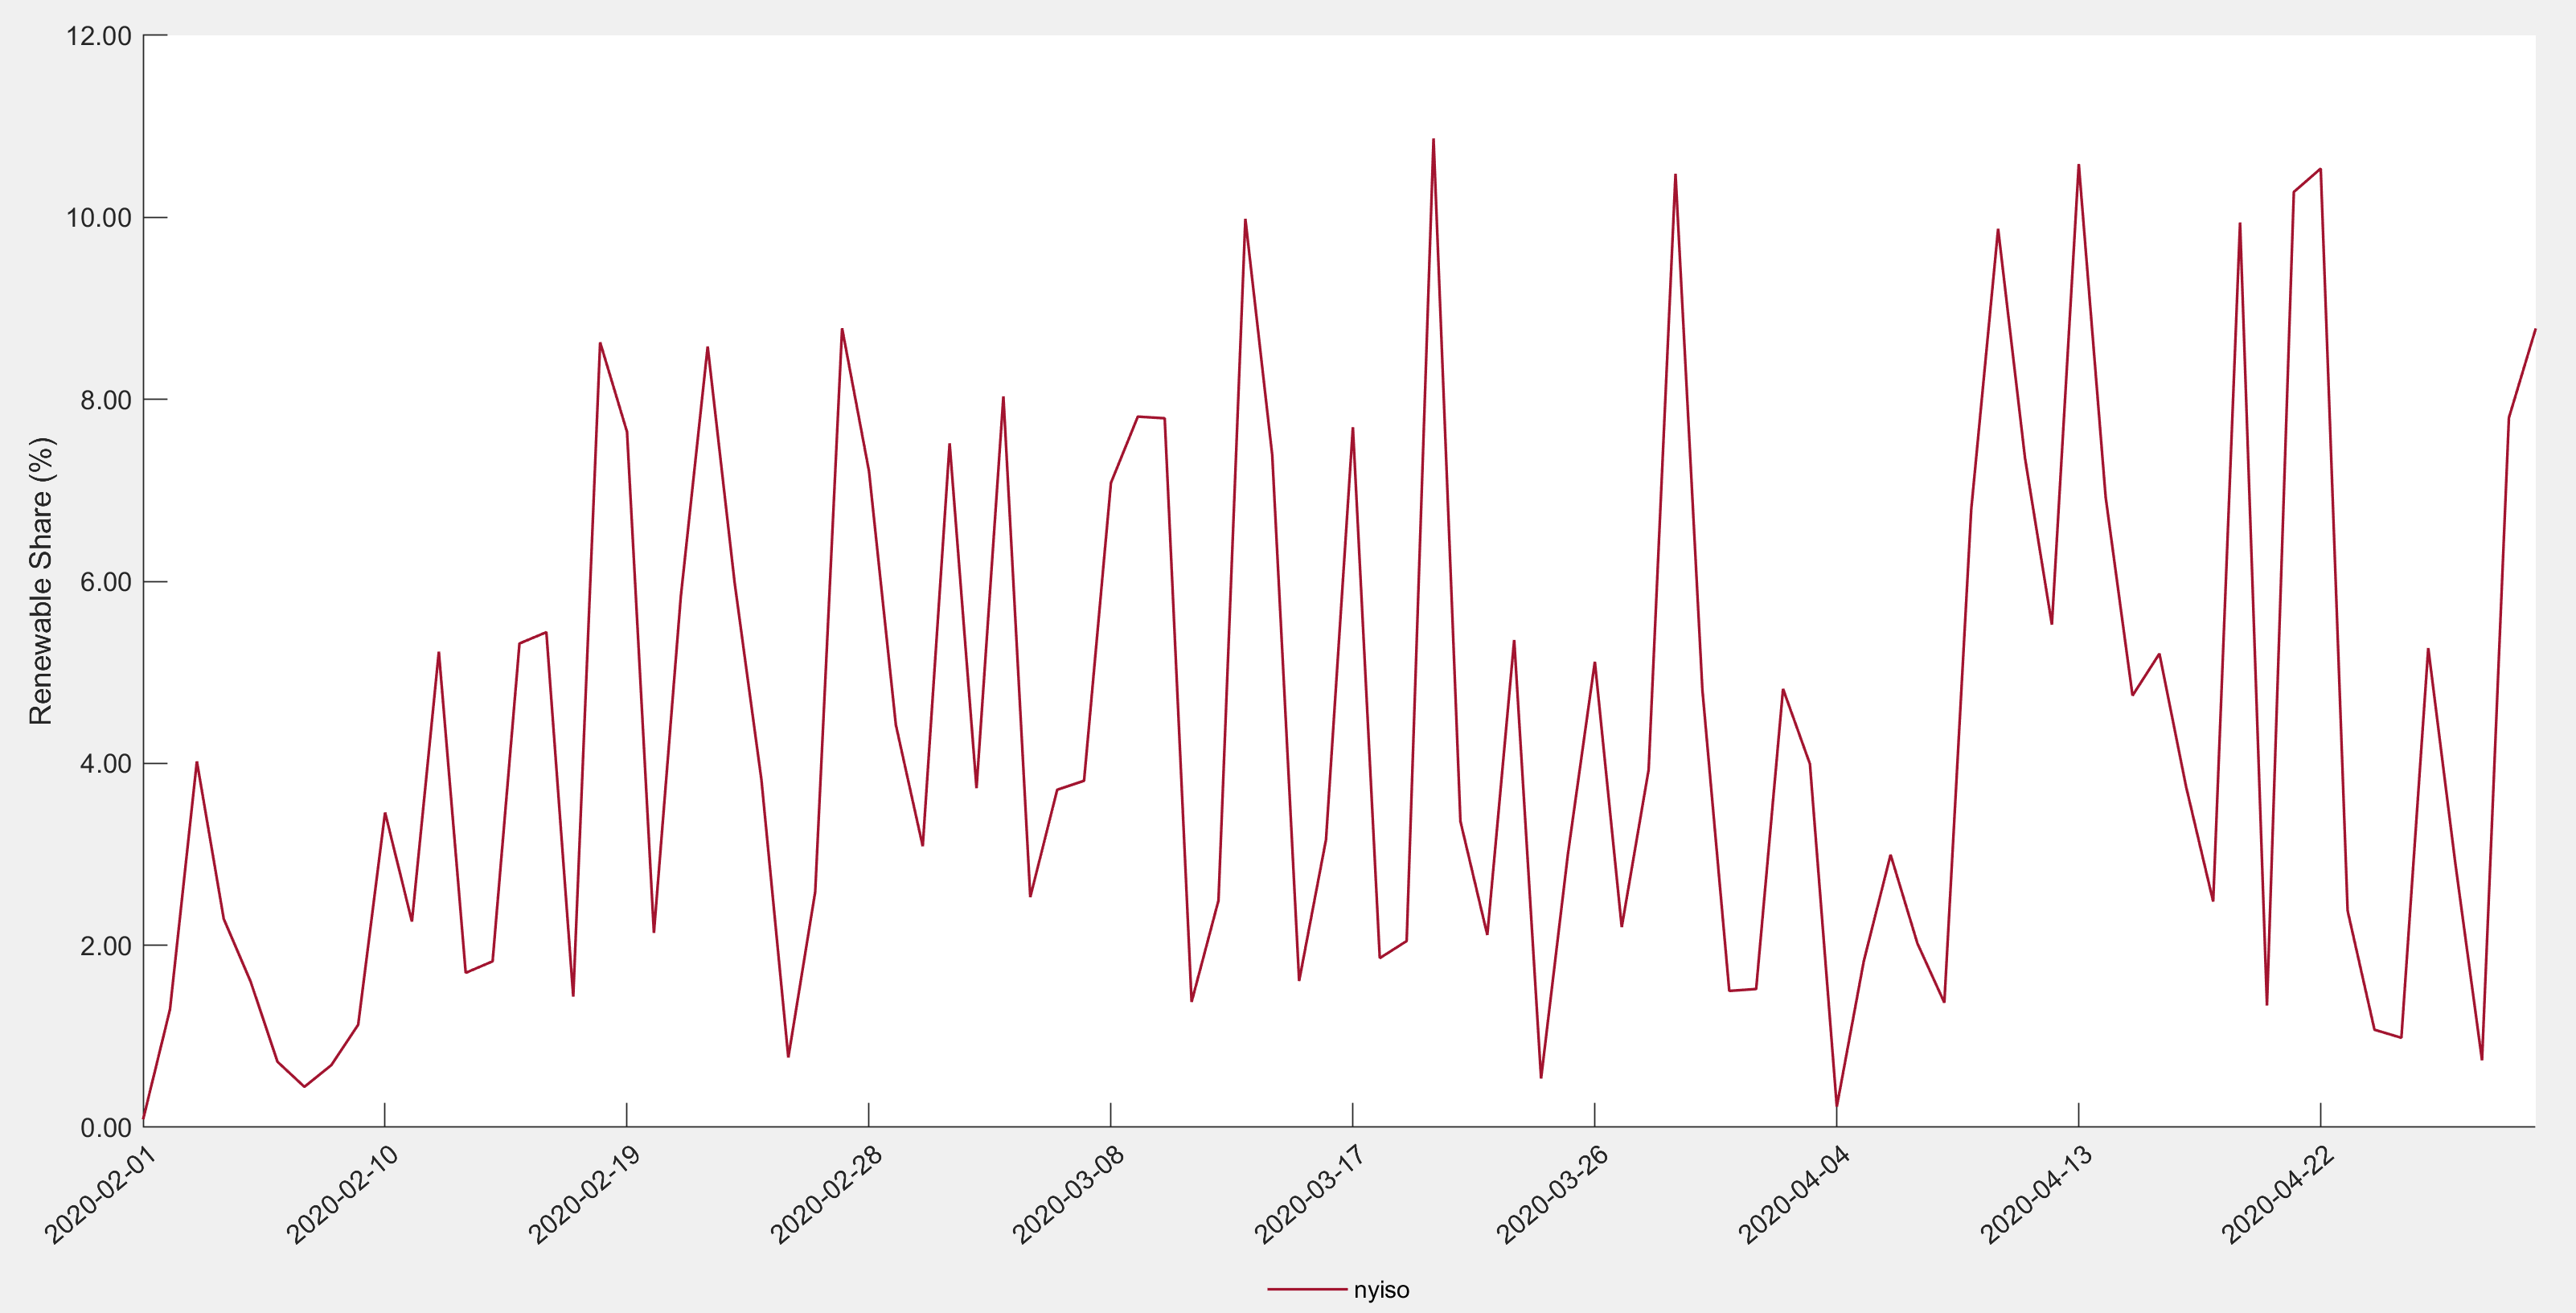
\includegraphics[width=\textwidth]{figures/plot_renewable_share_example3.jpg}
\end{center}

\subparagraph{Specify line properties}
Calculate the renewable share of NYISO. Display it in an line plot and change the Display name.

\begin{Code}
  plot_renewable_share('nyiso',...
  'DateRange', {'2020-02-01','2020-04-30'},...
  'DisplayName','2020','LineStyle', '--');
\end{Code}

\begin{center}
  \noindent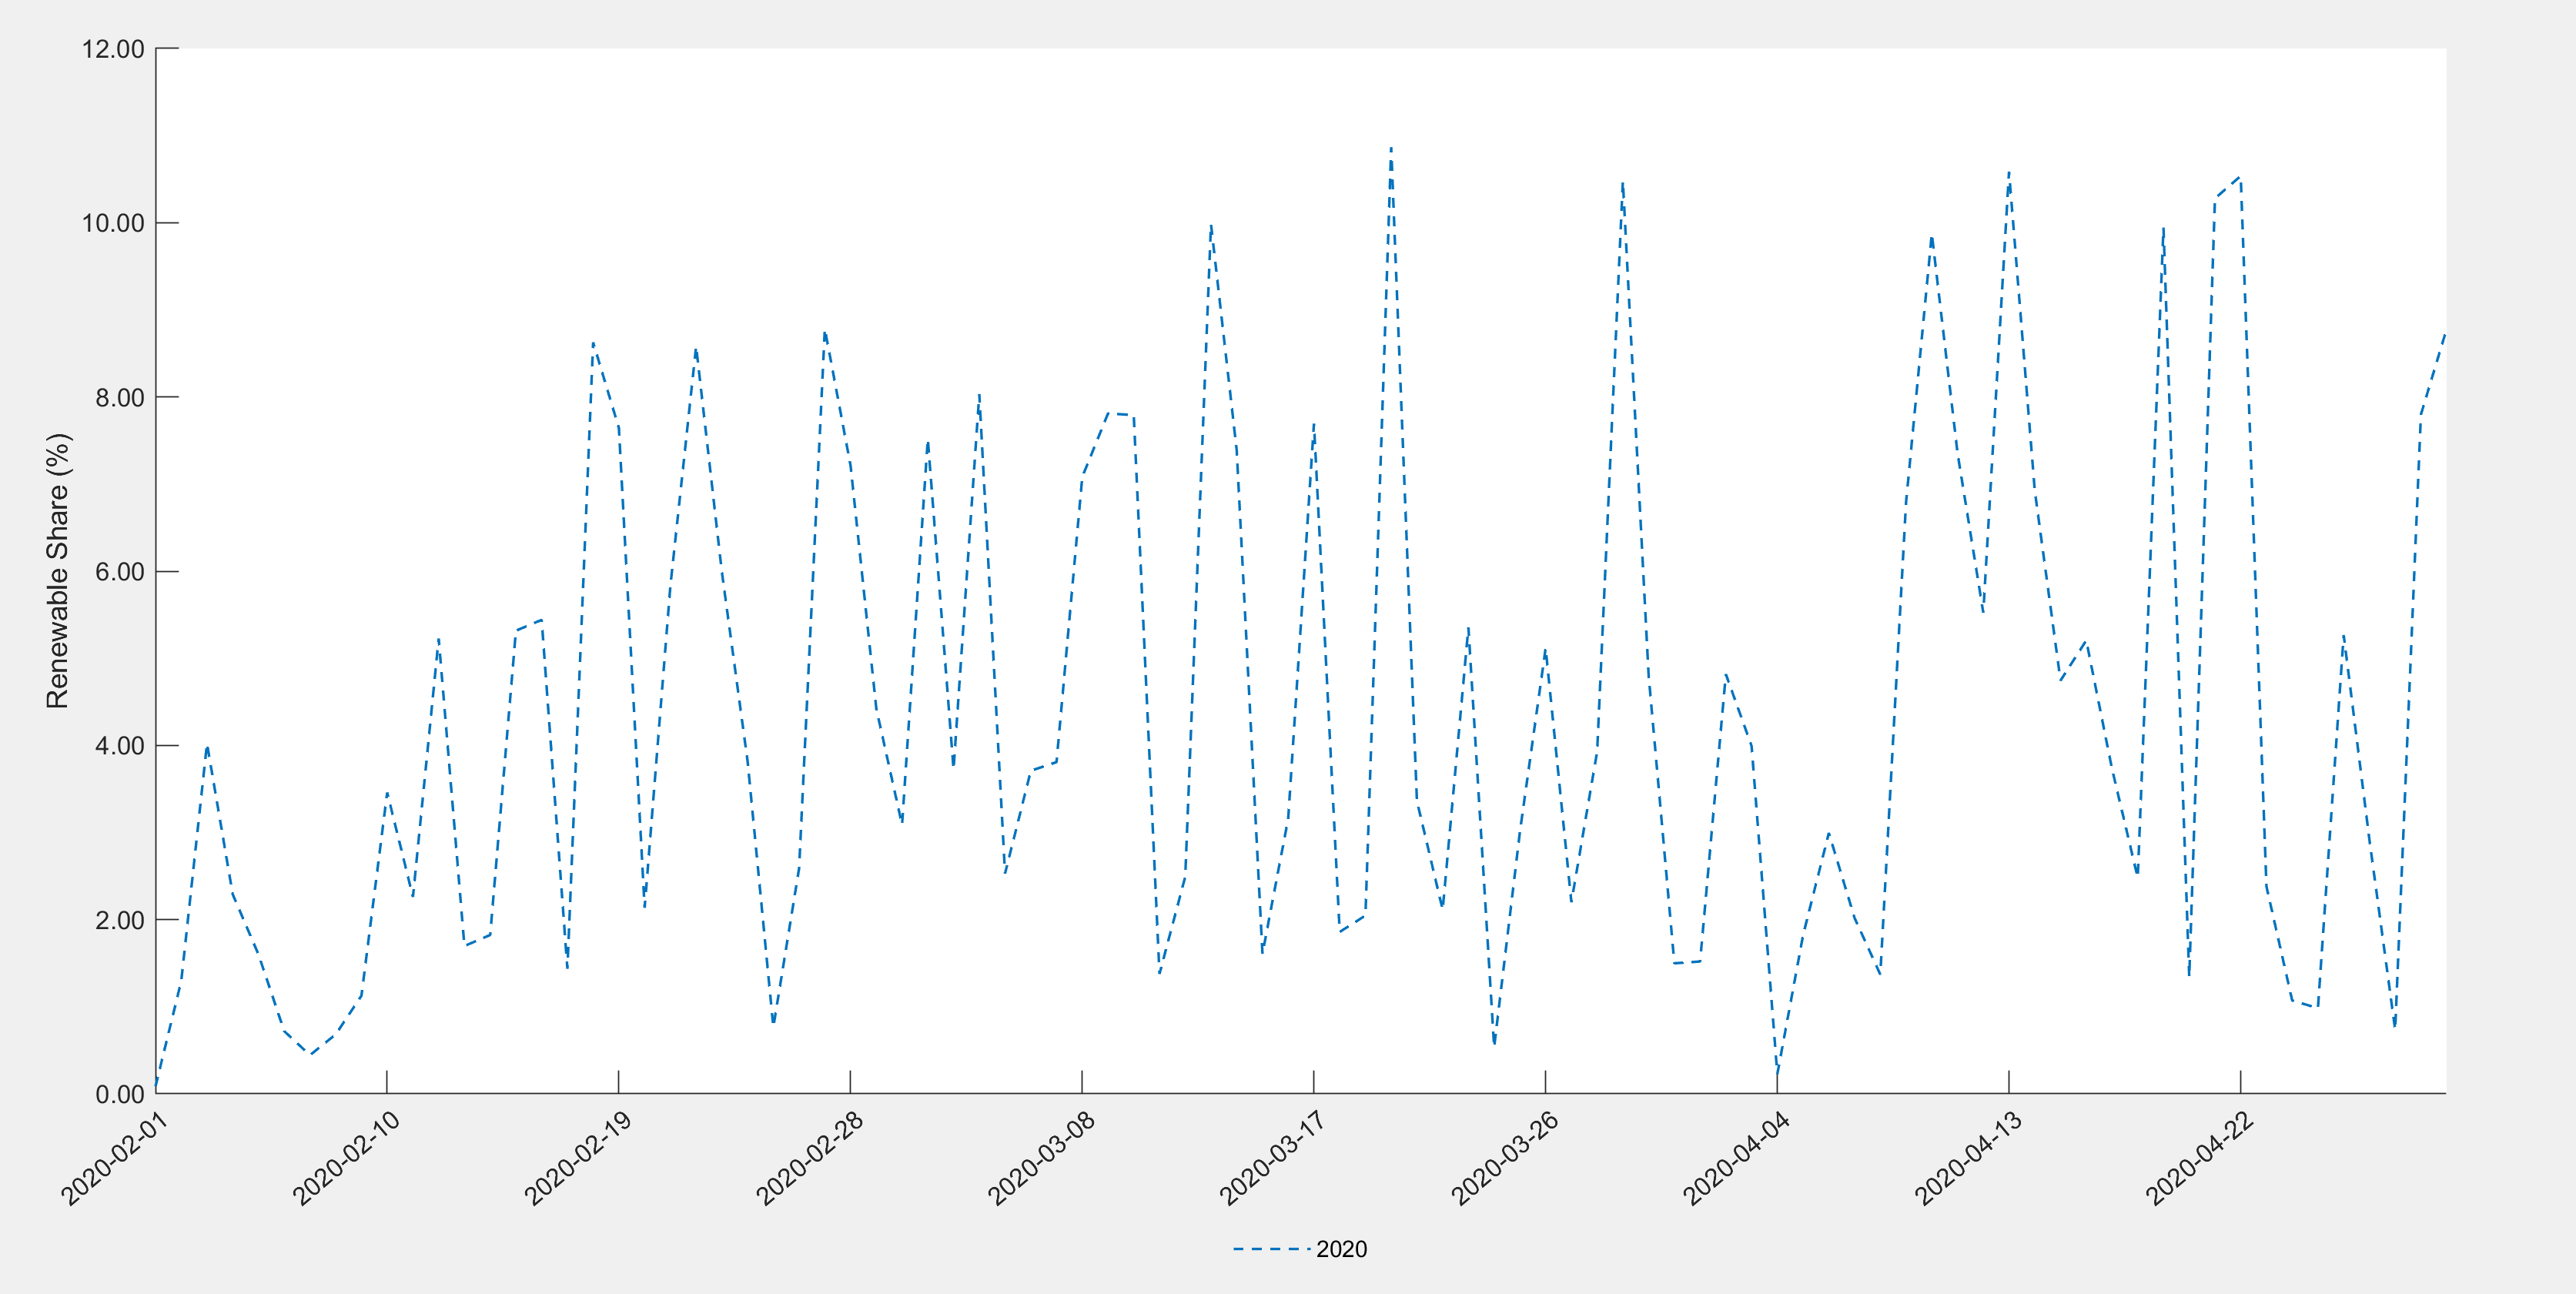
\includegraphics[width=\textwidth]{figures/plot_renewable_share_example4.jpg}
\end{center}

\subparagraph{Modify properties after plotting}
Calculate the renewable share of NYISO. Modify the properties of line objects and axes after displaying the plot.

\begin{Code}
  p = plot_renewable_share('nyiso');
  p.LineWidth = 2;
  ax = gca;
  ax.FontSize = 8;
\end{Code}

Note that users can customize the axes by using \verb!ax = gca!.

\begin{center}
  \noindent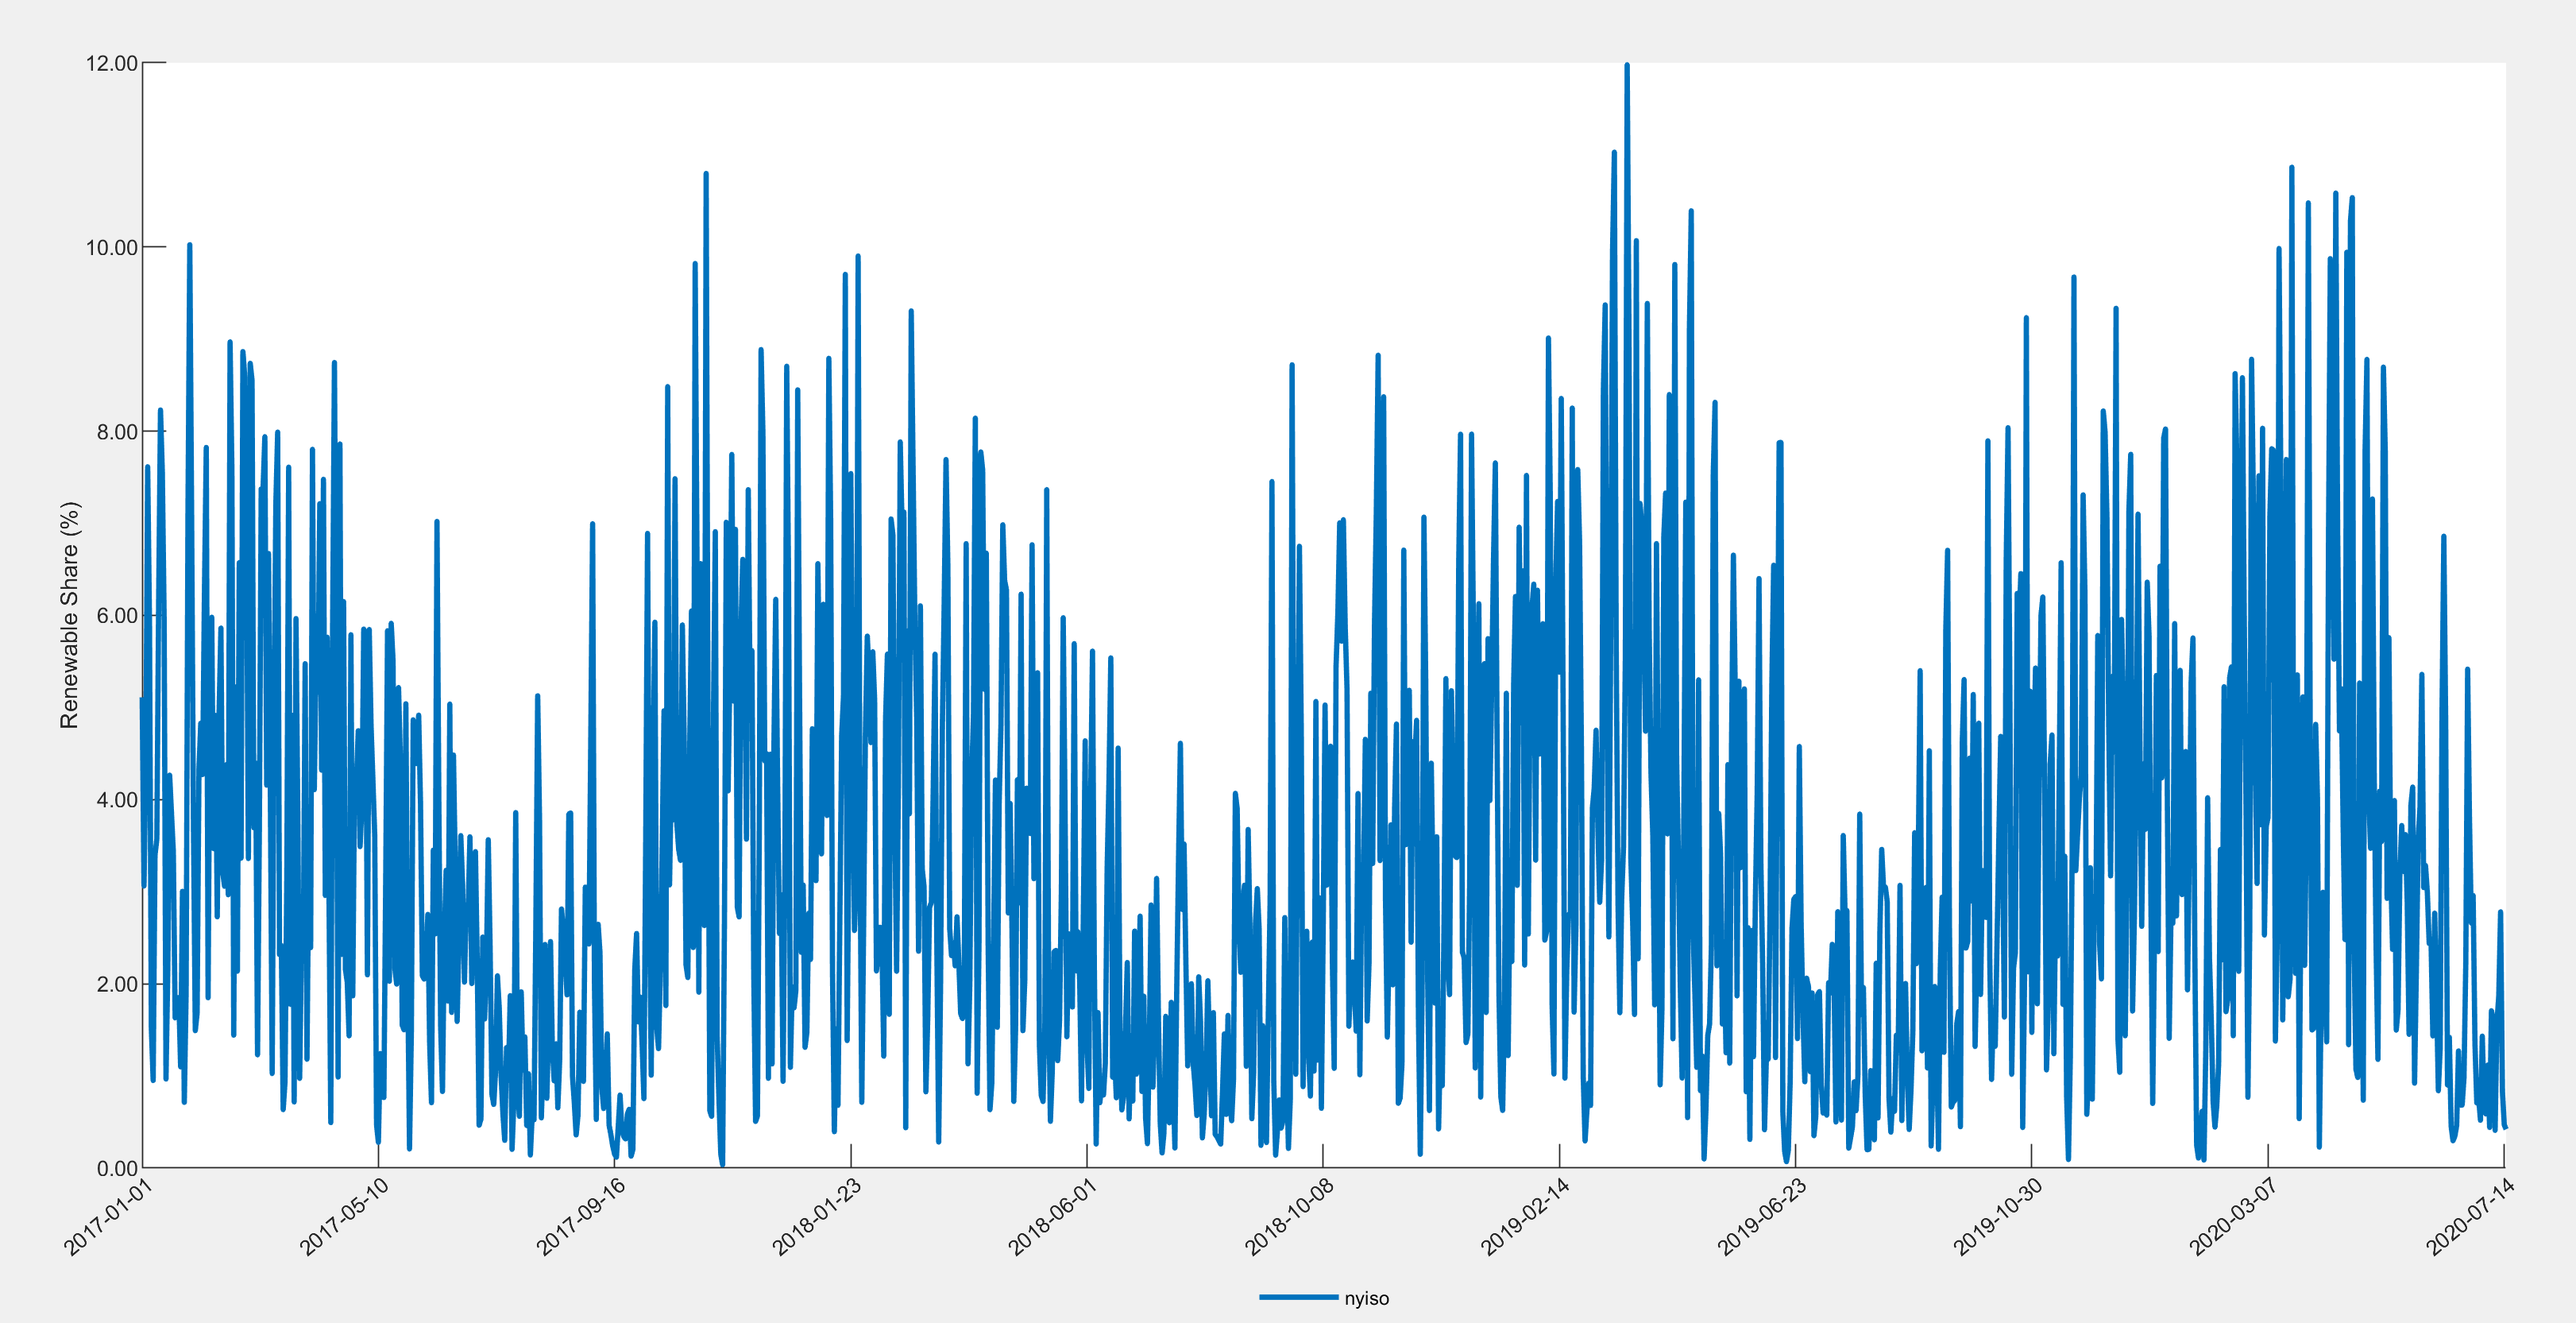
\includegraphics[width=\textwidth]{figures/plot_renewable_share_example5.jpg}
\end{center}




\subsection{Demand Profiles}
\subsubsection{plot demand}
\begin{Code}
  p = plot_demand(market, varargin)
\end{Code}

Plot the demand curve of a market.

Return the line object of the plot.

This function is based on \matlab{} function \verb!plot!.


\paragraph{Input Arguments}
\subparagraph{market:} \textit{character vectors}

Name of the market, specified as one of the seven market names:

\verb!'caiso' | 'ercot' | 'isone' | 'miso' | 'nyiso' | 'pjm' | 'spp'!

\paragraph{Name-Value Pair Arguments}
\subparagraph{DateRange:} \textit{datetime array $|$ string array $|$ cell array of character vectors}

Range of time, specified as a datetime array, a string array or a cell array of character vectors. Default \verb!{'2017-01-01','2020-07-15'}!.

Example: \verb!{'2017-01-01','2020-07-15'}!

Example: \verb!["2020-02-01","2020-04-30"]!

\subparagraph{ResampleBin:} \textit{string $|$ character vector}

Binning scheme for resampling. See also \verb!groupsummary!. Default \verb!'none'!.

\subparagraph{ResampleMethod:} \textit{string $|$ character vector}

Computation method for resampling. See also \verb!groupsummary!. Default \verb!'mean'!.

\subparagraph{Others:}

Modifications of the line object. See \verb!Line Properties!.



\paragraph{Output Arguments}
\subparagraph{p:} \textit{line object}

The line object of the plot. Use \verb!p! to modify properties of the line after creating it. See also \verb!Line Properties!.



\paragraph{Examples}
\subparagraph{Plot demand curve of a market}

Create a line plot of the demand of NYISO.

\begin{Code}
  plot_demand('nyiso');
\end{Code}

\begin{center}
  \noindent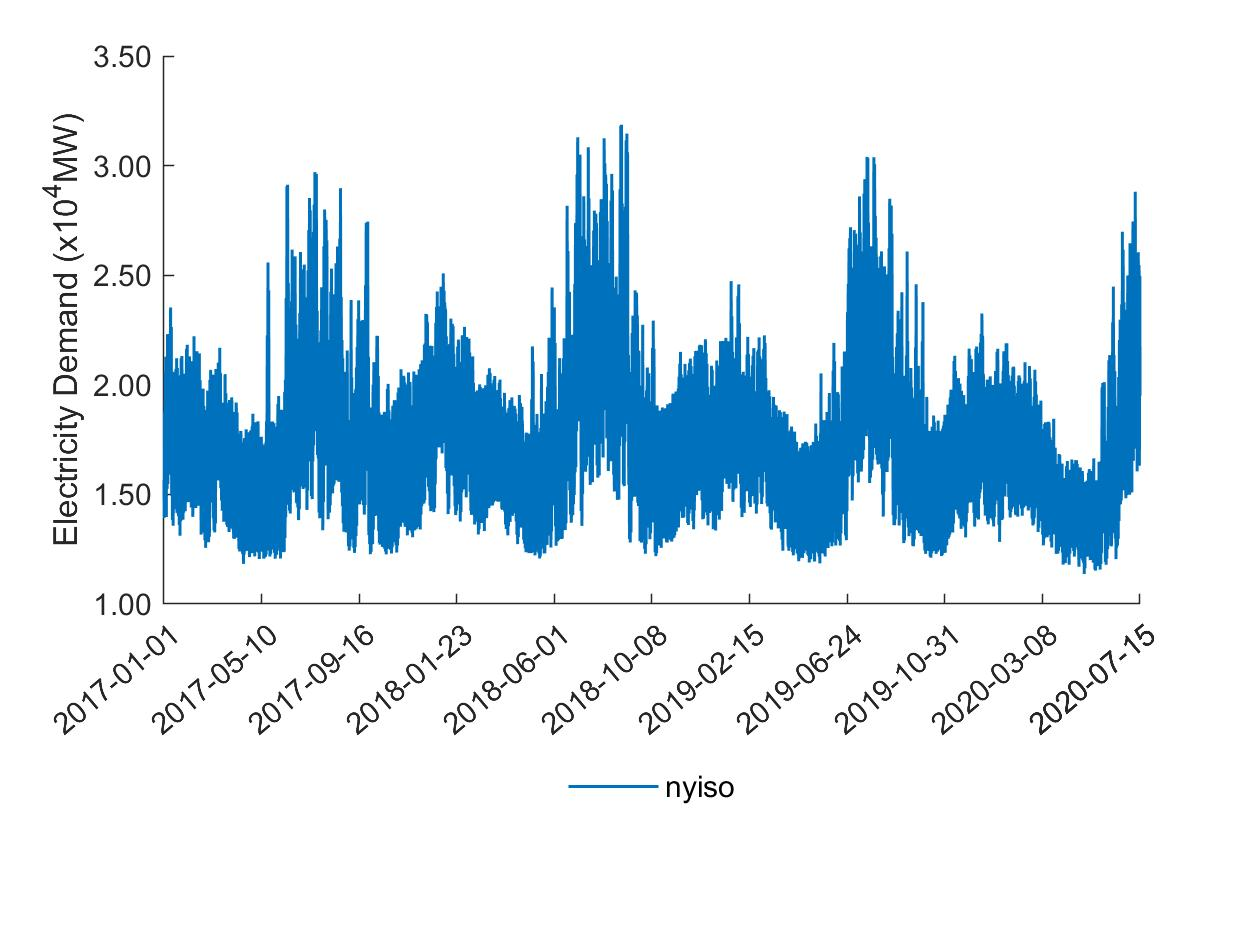
\includegraphics[width=\textwidth]{figures/plot_demand_example1.jpg}
\end{center}

\subparagraph{Customize binning scheme and computation method}

Calculate the total demand of NYISO every month in 2019. Display it in a line plot.

\begin{Code}
  plot_demand('nyiso', 'DateRange',...
  {'2019-01-01', '2019-12-31'},'ResampleBin',...
  'month', 'ResampleMethod', 'sum');
\end{Code}

\begin{center}
  \noindent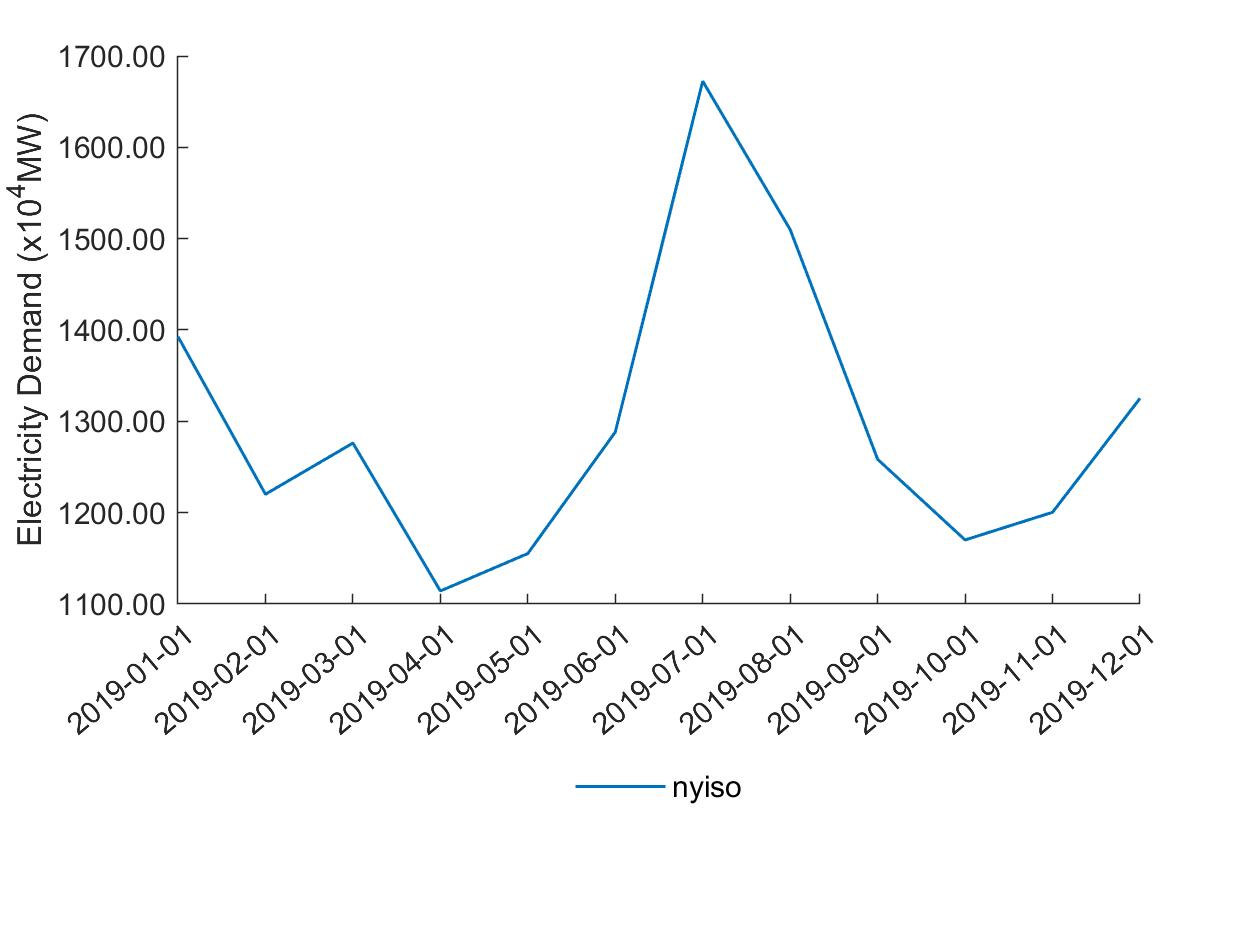
\includegraphics[width=\textwidth]{figures/plot_demand_example2.jpg}
\end{center}

\subparagraph{Specify line properties}
Create a line plot of the demand of NYISO. Set its legend, color and line width.

\begin{Code}
  plot_demand('nyiso', 'DateRange',...
  {'2020-02-01', '2020-04-30'}, 'DisplayName',...
  '2020', 'Color', '#0072BD', 'LineWidth', 2.5);
\end{Code}

\begin{center}
  \noindent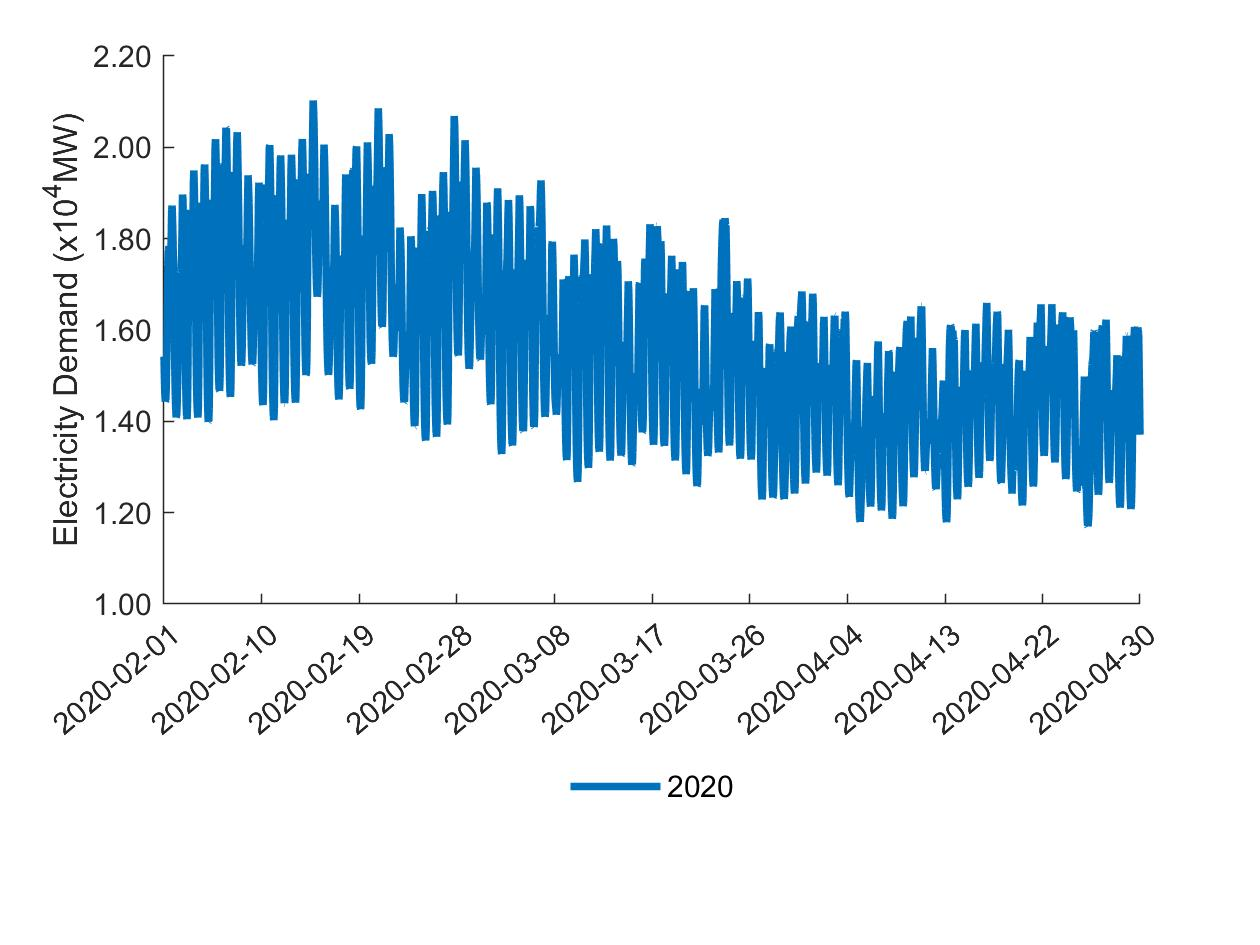
\includegraphics[width=\textwidth]{figures/plot_demand_example3.jpg}
\end{center}

\subparagraph{Modify properties after plotting}
Create a line plot of the demand of NYISO. Modify the properties of the line and axes after displaying the plot.

\begin{Code}
  p = plot_demand('nyiso', 'DateRange',...
  {'2020-02-01', '2020-04-30'});
  p.DisplayName = '2020';
  p.Color = '#0072BD';
  p.LineWidth = 2.5;
  ax = gca;
  ax.FontName = 'Consolas';
\end{Code}

For a list of properties, see \verb!Line Properties! and \verb!Axes Properties!.

\begin{center}
  \noindent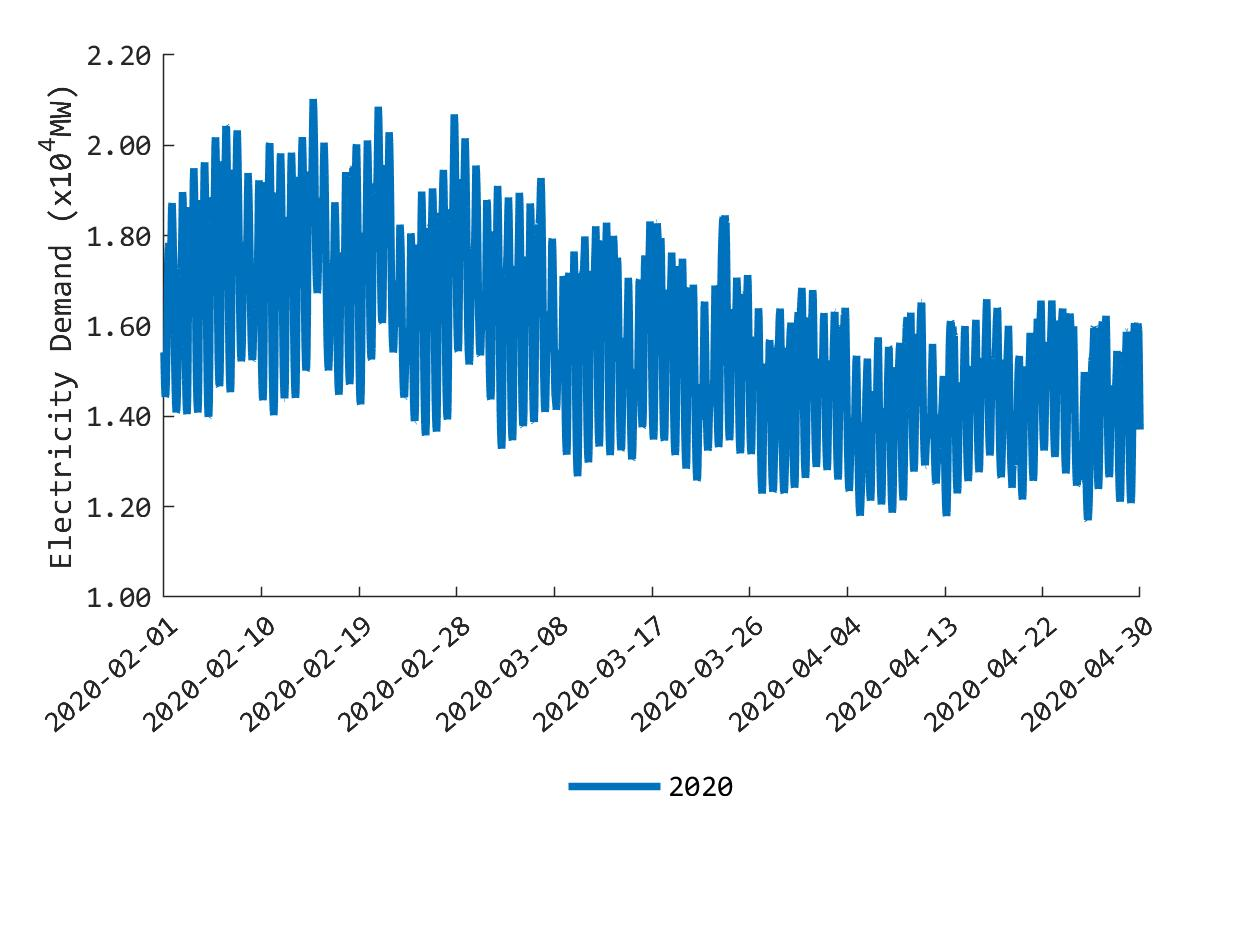
\includegraphics[width=\textwidth]{figures/plot_demand_example4.jpg}
\end{center}

\subparagraph{Plot multiple demand curves}
Plot the demand curves of NYISO in 2018, 2019 and 2020 with week alignment.

Calculate the corresponding date range.

\begin{Code}
  dr_2020 = datetime({'2020-02-01', '2020-04-30'});
  dw = calweeks(52);
  dr_2019 = dr_2020 - dw;
  dr_2018 = dr_2019 - dw;
\end{Code}

Plot the demand curves.

\begin{Code}
  plot_demand('nyiso', 'DateRange',...
  dr_2018, 'DisplayName', '2018',...
  'LineStyle', ':', 'Color', '#939598');
  plot_demand('nyiso', 'DateRange',...
  dr_2019, 'DisplayName', '2019',...
  'LineStyle', '--', 'Color', '#D95319');
  plot_demand('nyiso', 'DateRange',...
  dr_2020, 'DisplayName', '2020',...
  'Color', '#0072BD', 'LineWidth', 2.5);
\end{Code}

\begin{center}
  \noindent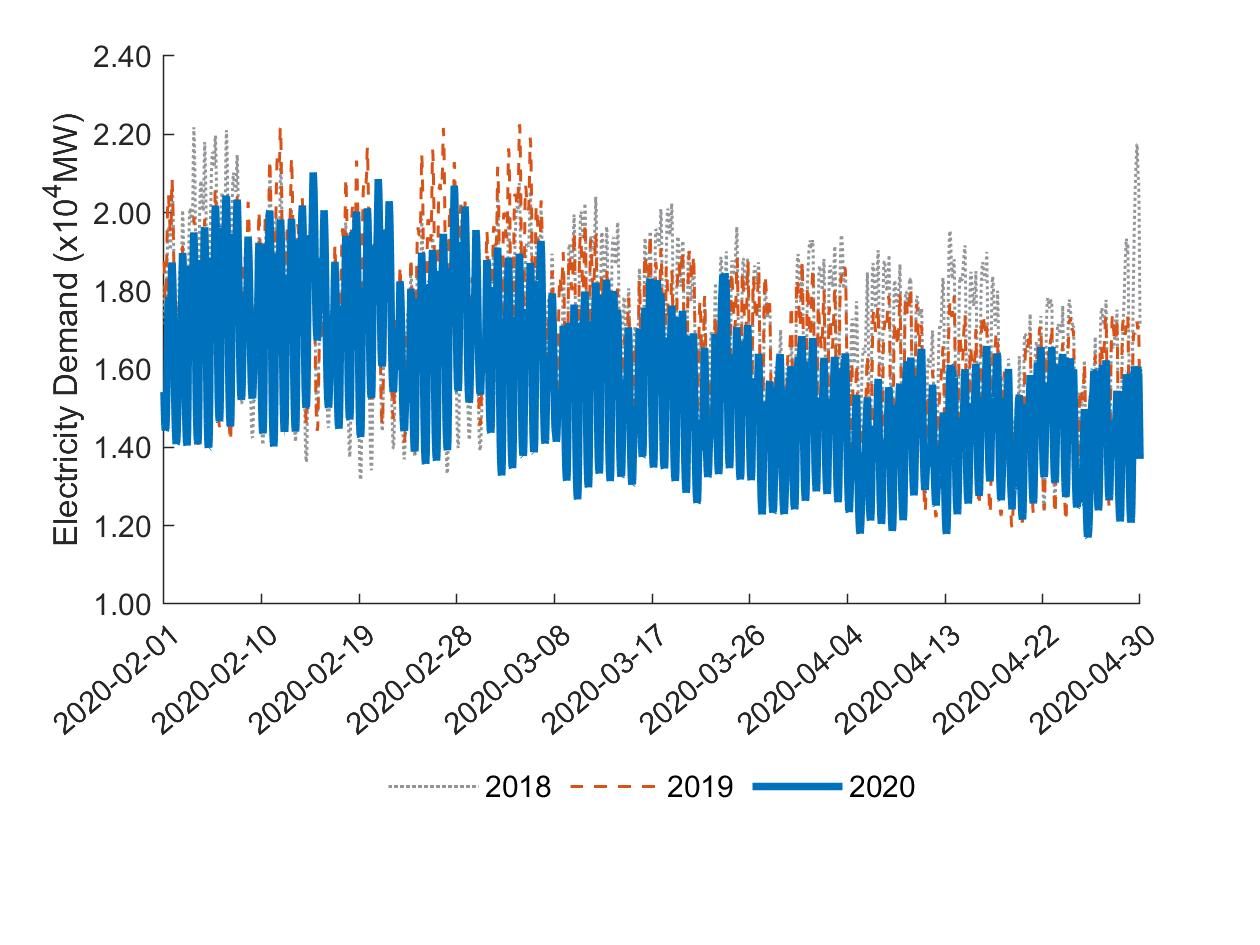
\includegraphics[width=\textwidth]{figures/plot_demand_example5.jpg}
\end{center}





\subsubsection{plot daily demand curve}
\begin{Code}
  ar = plot_daily_demand_curve(market, varargin)
\end{Code}

Plot the daily demand curve of a market with quantiles.

Return the area and line objects of the plot. If there are odd quantiles, the central one is displayed as a line object (\verb!plot!). Otherwise all of them are displayed as area objects (\verb!area!).

This function is based on \matlab{} function \verb!plot! and \verb!area!.


\paragraph{Input Arguments}
\subparagraph{market:} \textit{character vectors}

Name of the market, specified as one of the seven market names:

\verb!'caiso' | 'ercot' | 'isone' | 'miso' | 'nyiso' | 'pjm' | 'spp'!

\paragraph{Name-Value Pair Arguments}
\subparagraph{DateRange:} \textit{datetime array $|$ string array $|$ cell array of character vectors}

Range of time, specified as a datetime array, a string array or a cell array of character vectors. Default \verb!{'2017-01-01','2020-07-15'}!.

Example: \verb!{'2017-01-01','2020-07-15'}!

Example: \verb!["2020-02-01","2020-04-30"]!

\subparagraph{Quantile:} \textit{vector}

Cumulative probabilities for which to compute the quantiles. See also \verb!quantile!. Default \verb![0.05, 0.25, 0.5, 0.75, 0.95]!.

\subparagraph{Color:} \textit{RGB triplet $|$ hexadecimal color code \dots}

Color theme of the plot. This argument determines color of all the area and line objects in the plot. See \verb!Line Properties! and \verb!Area Properties!.

\subparagraph{Alpha:} \textit{vector}

Face transparency of the area objects. This argument determines transparency of all area ojects. See \verb!Line Properties! and \verb!Area Properties!. Default \verb![0.1, 0.25]!.

Example: \verb![0.1, 0.25]! (5 quantiles)

Example: \verb![0, 0.1, 0.25]! (5 quantiles)

Example: \verb![0.1, 0.25, 0.1]! (5 quantiles)

Example: \verb![0, 0.1, 0.25, 0.1]! (5 quantiles)

All the examples above have the same effect.

Example: \verb![0.1, 0.25]! (6 quantiles)

Example: \verb![0, 0.1, 0.25]! (6 quantiles)

Example: \verb![0.1, 0.25, 1]! (6 quantiles)

Example: \verb![0, 0.1, 0.25, 1]! (6 quantiles)

Example: \verb![0.1, 0.25, 1, 0.25, 0.1]! (6 quantiles)

Example: \verb![0, 0.1, 0.25, 1, 0.25, 0.1]! (6 quantiles)

All the examples above have the same effect.

\subparagraph{LineWidth:} \textit{scalar numeric value}

Line width of the central line (if exists). See \verb!Line Properties!.

\underline{Note: To further adjust the plot, modify properties of the objects after creating them.}



\paragraph{Output Arguments}
\subparagraph{ar:} \textit{area objects and line object (optional)}

Area objects and the line object (if exists) of the plot. The number of objects is equal to the number of quantiles. Use \verb!ar! to modify properties after creating them. See also \verb!Area Properties! and \verb!Line Properties!.



\paragraph{Examples}
\subparagraph{Plot daily demand curve of a market}

Calculate the daily demand curve of NYISO. Display it in a plot.

\begin{Code}
  plot_daily_demand_curve('nyiso');
\end{Code}

\begin{center}
  \noindent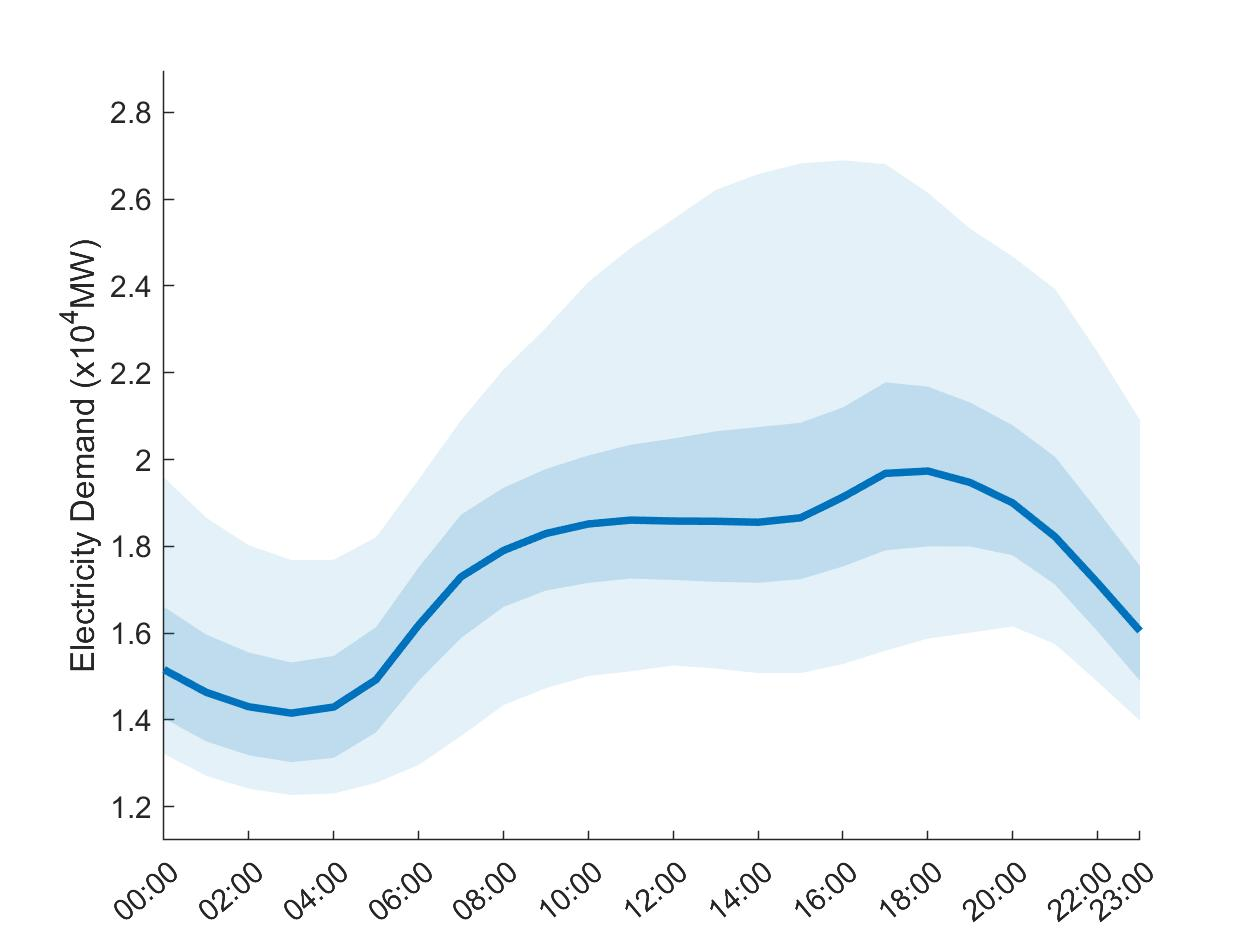
\includegraphics[width=\textwidth]{figures/plot_daily_demand_curve_example1.jpg}
\end{center}



\subparagraph{Customize date range and quantiles}

Calculate the daily demand curve of NYISO in Feb-2018 with quantiles set as [0.05, 0.15, 0.45, 0.65, 0.85, 0.95]. Display it in a plot.

\begin{Code}
  plot_daily_demand_curve('nyiso', 'DateRange',...
  {'2018-02-01', '2018-02-28'}, 'Quantile',...
  [0.05, 0.15, 0.45, 0.55, 0.85, 0.95]);
\end{Code}

\begin{center}
  \noindent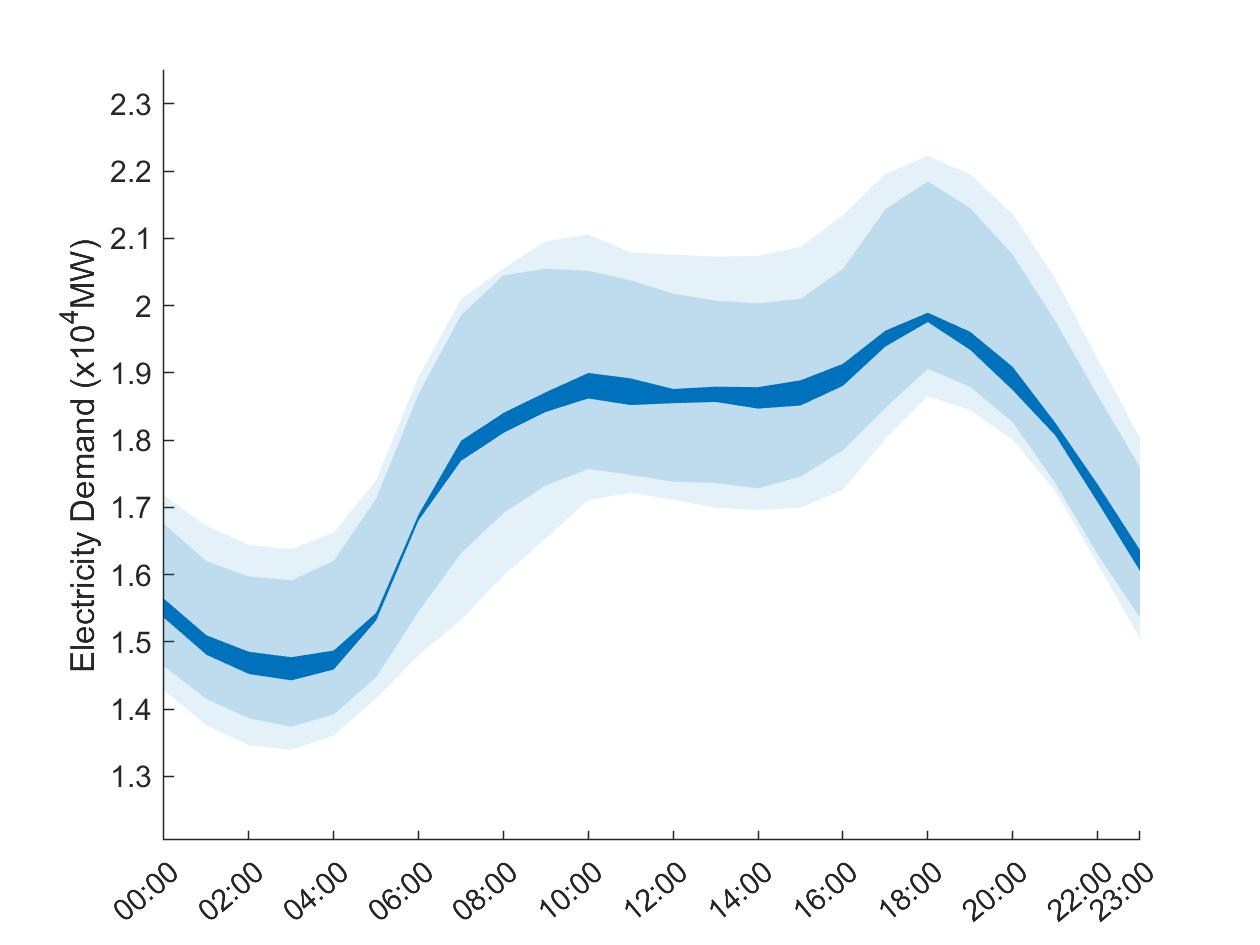
\includegraphics[width=\textwidth]{figures/plot_daily_demand_curve_example2.jpg}
\end{center}



\subparagraph{Specify area and line properties}

Calculate the daily demand curve of NYISO. Display it in a plot. Set its color, transparency and line width.

\begin{Code}
  plot_daily_demand_curve('nyiso', 'Color', 'b',...
  'Alpha', [0.2, 0.5], 'LineWidth', 5);
\end{Code}

\begin{center}
  \noindent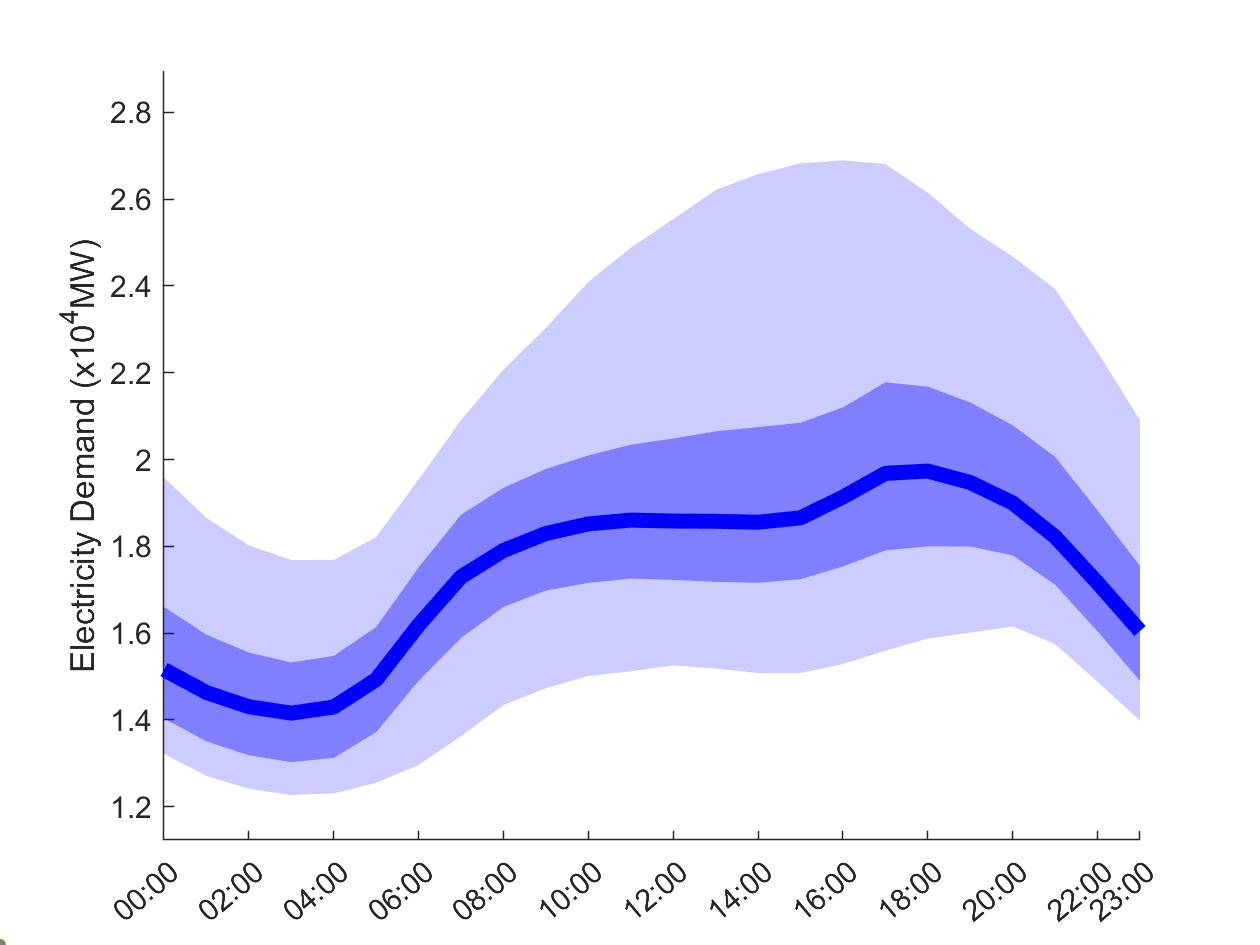
\includegraphics[width=\textwidth]{figures/plot_daily_demand_curve_example3.jpg}
\end{center}





\subsection{Price Distribution}

\subsection{Mobility}






%--------------------------------
\newpage
\section{Baseline Estimation} \label{sec:baseline}

\subsection{Date and Week Alignment}

\subsection{Ensemble Backcast Estimation}

\subsection{Abnormal Price Index}

\subsection{Excess Change Rate of Renewable}





%---------------------------------
\newpage
\section{Regression Analysis} \label{sec:regression}

\subsection{Regression Methodology}

\subsection{Factor Analysis}






%------------------------------------------------
\newpage
\section{Acknowledgments} \label{sec:thanks}






%------------------------------------------------
\begin{appendices}

\newpage
\section{Glossary} \label{sec:}


\end{appendices}




\newpage
\section*{Reference} \label{sec:ref}
\addcontentsline{toc}{section}{Reference}

\end{document}
